\documentclass{fun_article}

\title{Attention before agreement forecasts the focus of soft-law action}
\definecolor{orcidlogocol}{HTML}{A6CE39}

\author[*, 1, 2, 3]{Casper van Elteren\orcid{0000-0001-9862-8936}}
\author[5]{Fiona Lippert\orcid{0000-0003-4174-2230}}
\author[1]{Zach Carter\orcid{0000-0002-0709-4412}}
\author[1]{Maria Kleshnina\orcid{0000-0002-5518-8317}}
\author[1]{Michael Bode\orcid{0000-0002-5886-4421}}
\author[3, 4]{Vítor V. Vasconcelos\orcid{0000-0002-4621-5272}}

\renewcommand\Affilfont{\small}
\affil[*]{Corresponding author: casper.vanelteren@qut.edu.au}
\affil[1]{Securing Antarctica's Environmental Future, School of Mathematics, Queensland University of Technology, Brisbane, Australia}
\affil[2]{Institute for Advanced Study, University of Amsterdam, 1012 GC Amsterdam, Netherlands}
\affil[3]{Computational Science Lab, Informatics Institute, University of Amsterdam, 1090 GH Amsterdam, The Netherlands}
\affil[4]{Polder Center, Institute for Advanced Study, University of Amsterdam, 1012 GC Amsterdam, The Netherlands}
\affil[5]{Space Research Organization Netherlands, 2333 CA Leiden, The Netherlands}
\addbibresource{theSpaceOfConcerns.bib}

\makeatletter
\@ifundefined{if@kernel@version@MMXXV}{\newif\if@kernel@version@MMXXV}{}
\let\@setmarks\@empty
\makeatother

\makeatletter
\renewcommand{\topfraction}{0.95}
\renewcommand{\dbltopfraction}{0.95}
\renewcommand{\textfraction}{0.05}
\renewcommand{\floatpagefraction}{0.8}
\renewcommand{\dblfloatpagefraction}{0.8}
\setcounter{topnumber}{2}
\setcounter{dbltopnumber}{2}
\setcounter{totalnumber}{4}
\setlength{\@fptop}{0pt}
\setlength{\@dblfptop}{0pt}
\makeatother

\makeatletter
\begin{document}
\makeatother
\sloppy
\begin{abstract}
Before a consensus institution can act on a new problem, participants must make room for it in a crowded agenda. That formative stage is rarely visible. We analyse 6,573 papers from more than six decades of Antarctic Treaty meetings alongside the complete record of Measures, Decisions, and Resolutions adopted at regular meetings since 1995. We place concerns close when the same actors devote a disproportionate share of their papers to both. Actors move through this space locally: concerns near their earlier portfolios are more likely to become new specializations, and the shifts that occur are closer than issue popularity alone predicts. The map helps forecast formal output, but not uniformly. Combining papers on a concern with attention to related concerns improves rolling-origin forecasts of the issues addressed by non-binding Resolutions in 15 of 19 meetings, and the observed map outperforms every shuffled version. The same approach does not improve forecasts of Measures or Decisions. Measures instead remain concentrated in recurring work and usually cite earlier formal instruments. These findings separate movement in the agenda from continuity in formal action. Concern networks show where attention is likely to move and where it helps locate soft-law output, while potentially binding Measures remain anchored in a narrower record of earlier formal work.
\end{abstract}

\noindent\textbf{Keywords:} agenda formation, consensus governance, global commons, environmental governance, space of concerns, network analysis, Antarctic Treaty

\vspace{1em}
\noindent\textbf{Highlights}
\begin{itemize}
 \item Treaty papers reveal how institutional concerns share actors' attention
 \item Actors shift attention toward concerns close to their earlier portfolios
 \item Paper attention improves forecasts of non-binding Resolution topics
 \item Measures usually cite earlier formal outputs, especially Measures
\end{itemize}

\vspace{1em}
\noindent\textbf{Science for Society}
\newline
Before governments can agree on a response, they must decide where to spend limited time and expertise. More than six decades of Antarctic Treaty papers show that participants usually move toward concerns close to their earlier work. After model settings were fixed using earlier meetings, papers on the focal concern and network-weighted attention improved forecasts of the non-binding Resolutions adopted at later meetings. The same model did not improve forecasts of Measures or Decisions. Measures are concentrated in protected-area management and usually cite earlier formal outputs, especially earlier Measures. Monitoring concern networks can therefore give consensus institutions an early view of where attention is moving. Formal inheritance, legal status, implementation, and environmental outcomes then show how far institutional adaptation proceeds.

\section{Introduction}
Formal decisions create the governance record, but their orderly sequence can make the history of governance appear cleaner and more linear than it was. Those decisions compress conflict and shifts in attention, leaving much of the process out of view \cite{BachrachBaratz1962,Stone2013,Drubel2023HiddenContestation}. The work behind a decision begins earlier, as participants decide where to invest limited attention and expertise \cite{Kingdon1984,BaumgartnerJones1993,JonesBaumgartner2005,CoenEtAl2022}. We ask how that attention develops in the governance of a global commons and whether it helps forecast adopted formal output.

Research on institutional performance distinguishes process, policy output, and outcome. It also shows that international organizations can matter most near the start of the policy process \cite{GutnerThompson2010,CoenEtAl2022,BurchEtAl2019}. Agenda studies trace how attention rises and falls \cite{BaumgartnerJones1993,JonesBaumgartner2005,GreenPedersenWalgrave2014}. Network studies map relations among environmental agreements and organizations \cite{Kim2013,Kim2020}. These approaches leave unresolved which concerns occupy the same portfolios inside one institution, where actors direct attention next, and whether those relations appear in adopted output.

Answering this question requires a record that begins before agreement and can be followed into distinct forms of formal output. Consensus makes such a record especially valuable. Without roll calls, adoption does not reveal how strongly participants supported a text, and agreement may be secured by narrowing or weakening what the text requires \cite{Steinberg2002,Drubel2023HiddenContestation}. Outputs can also differ in legal force \cite{AbbottSnidal2000}. We therefore need an institution that preserves work before agreement and distinguishes among the forms that agreement takes.

The Antarctic Treaty system (ATS) provides this combination. Its consultative meetings have governed Antarctica by consensus since 1961 under a Treaty that reserves the continent for peaceful purposes \cite{Joyner1998,AntarcticTreaty1959,Yao2021}. Research on the ATS has already used submitted papers to examine participation, leadership, and institutional performance \cite{DudeneyWalton2012,Sanchez2016,Gardiner2025}. Participants use these papers to raise problems, present evidence, and propose action \cite{Kennicutt2019,Sampaio2022}. Since 1995, adopted outputs have been recorded as Resolutions, Decisions, or Measures. Resolutions are non-binding, Decisions organize internal work, and Measures can become legally binding after the required approvals. The ATS therefore provides a long record of documentary inputs alongside outputs with different legal consequences within one consensus institution.

We analyse 6,573 working papers and information documents submitted between 1961 and 2025 by 66 state and institutional actors. Preparing a paper uses limited time and resources, so the distribution of these documents records where participants place documentary effort. It cannot tell us whether that effort reflects strategy, mandate, expertise, or reporting duties. The Secretariat-maintained database returns the papers under 45 harmonized categories. Of the papers, 1,228 appear under two to five categories. A paper with $k$ categories contributes $1/k$ to each. This preserves the archive as returned instead of forcing an unobserved primary label (Methods and Supplementary Information \cref{fig:topic-submission-overview}).

From these records, we construct a \emph{space of concerns}. Two concerns are close when the same actors devote an above-average share of their papers to both. In plain terms, an actor is specialized when a concern occupies a larger share of its papers than that concern occupies across the archive. The map captures shared patterns of documentary attention, not collaboration, causal pathways, or similarity in wording. It lets us ask whether an actor's earlier portfolio predicts where its relative attention shifts next. We then aggregate papers to the broader categories used for adopted outputs and test whether direct and network-weighted attention improve rolling-origin forecasts of Measures, Decisions, and Resolutions. This adapts measures of relatedness used to study movement among products, industries, technologies, and research fields \cite{Hidalgo2007,Hidalgo2018,Neffke2011,Boschma2017,Guevara2016}. The concerns remain institutional categories, including procedural and administrative subjects that need not produce a separate output.

We use the same geometry at two levels. First, it predicts where individual portfolios shift. Second, after papers are aggregated across actors and categories, it tests whether the distribution of documentary attention helps forecast adopted output. Earlier portfolios narrow where actors shift relative effort. Direct and network-weighted attention improve rolling-origin forecasts of non-binding Resolutions, but not Measures or Decisions. Measures are concentrated in recurring area-management work and usually cite earlier formal outputs. Together, these analyses link the organization of attention to soft-law output and distinguish it from the formal inheritance seen in Measures.

\begin{figure*}[!t]
\centering 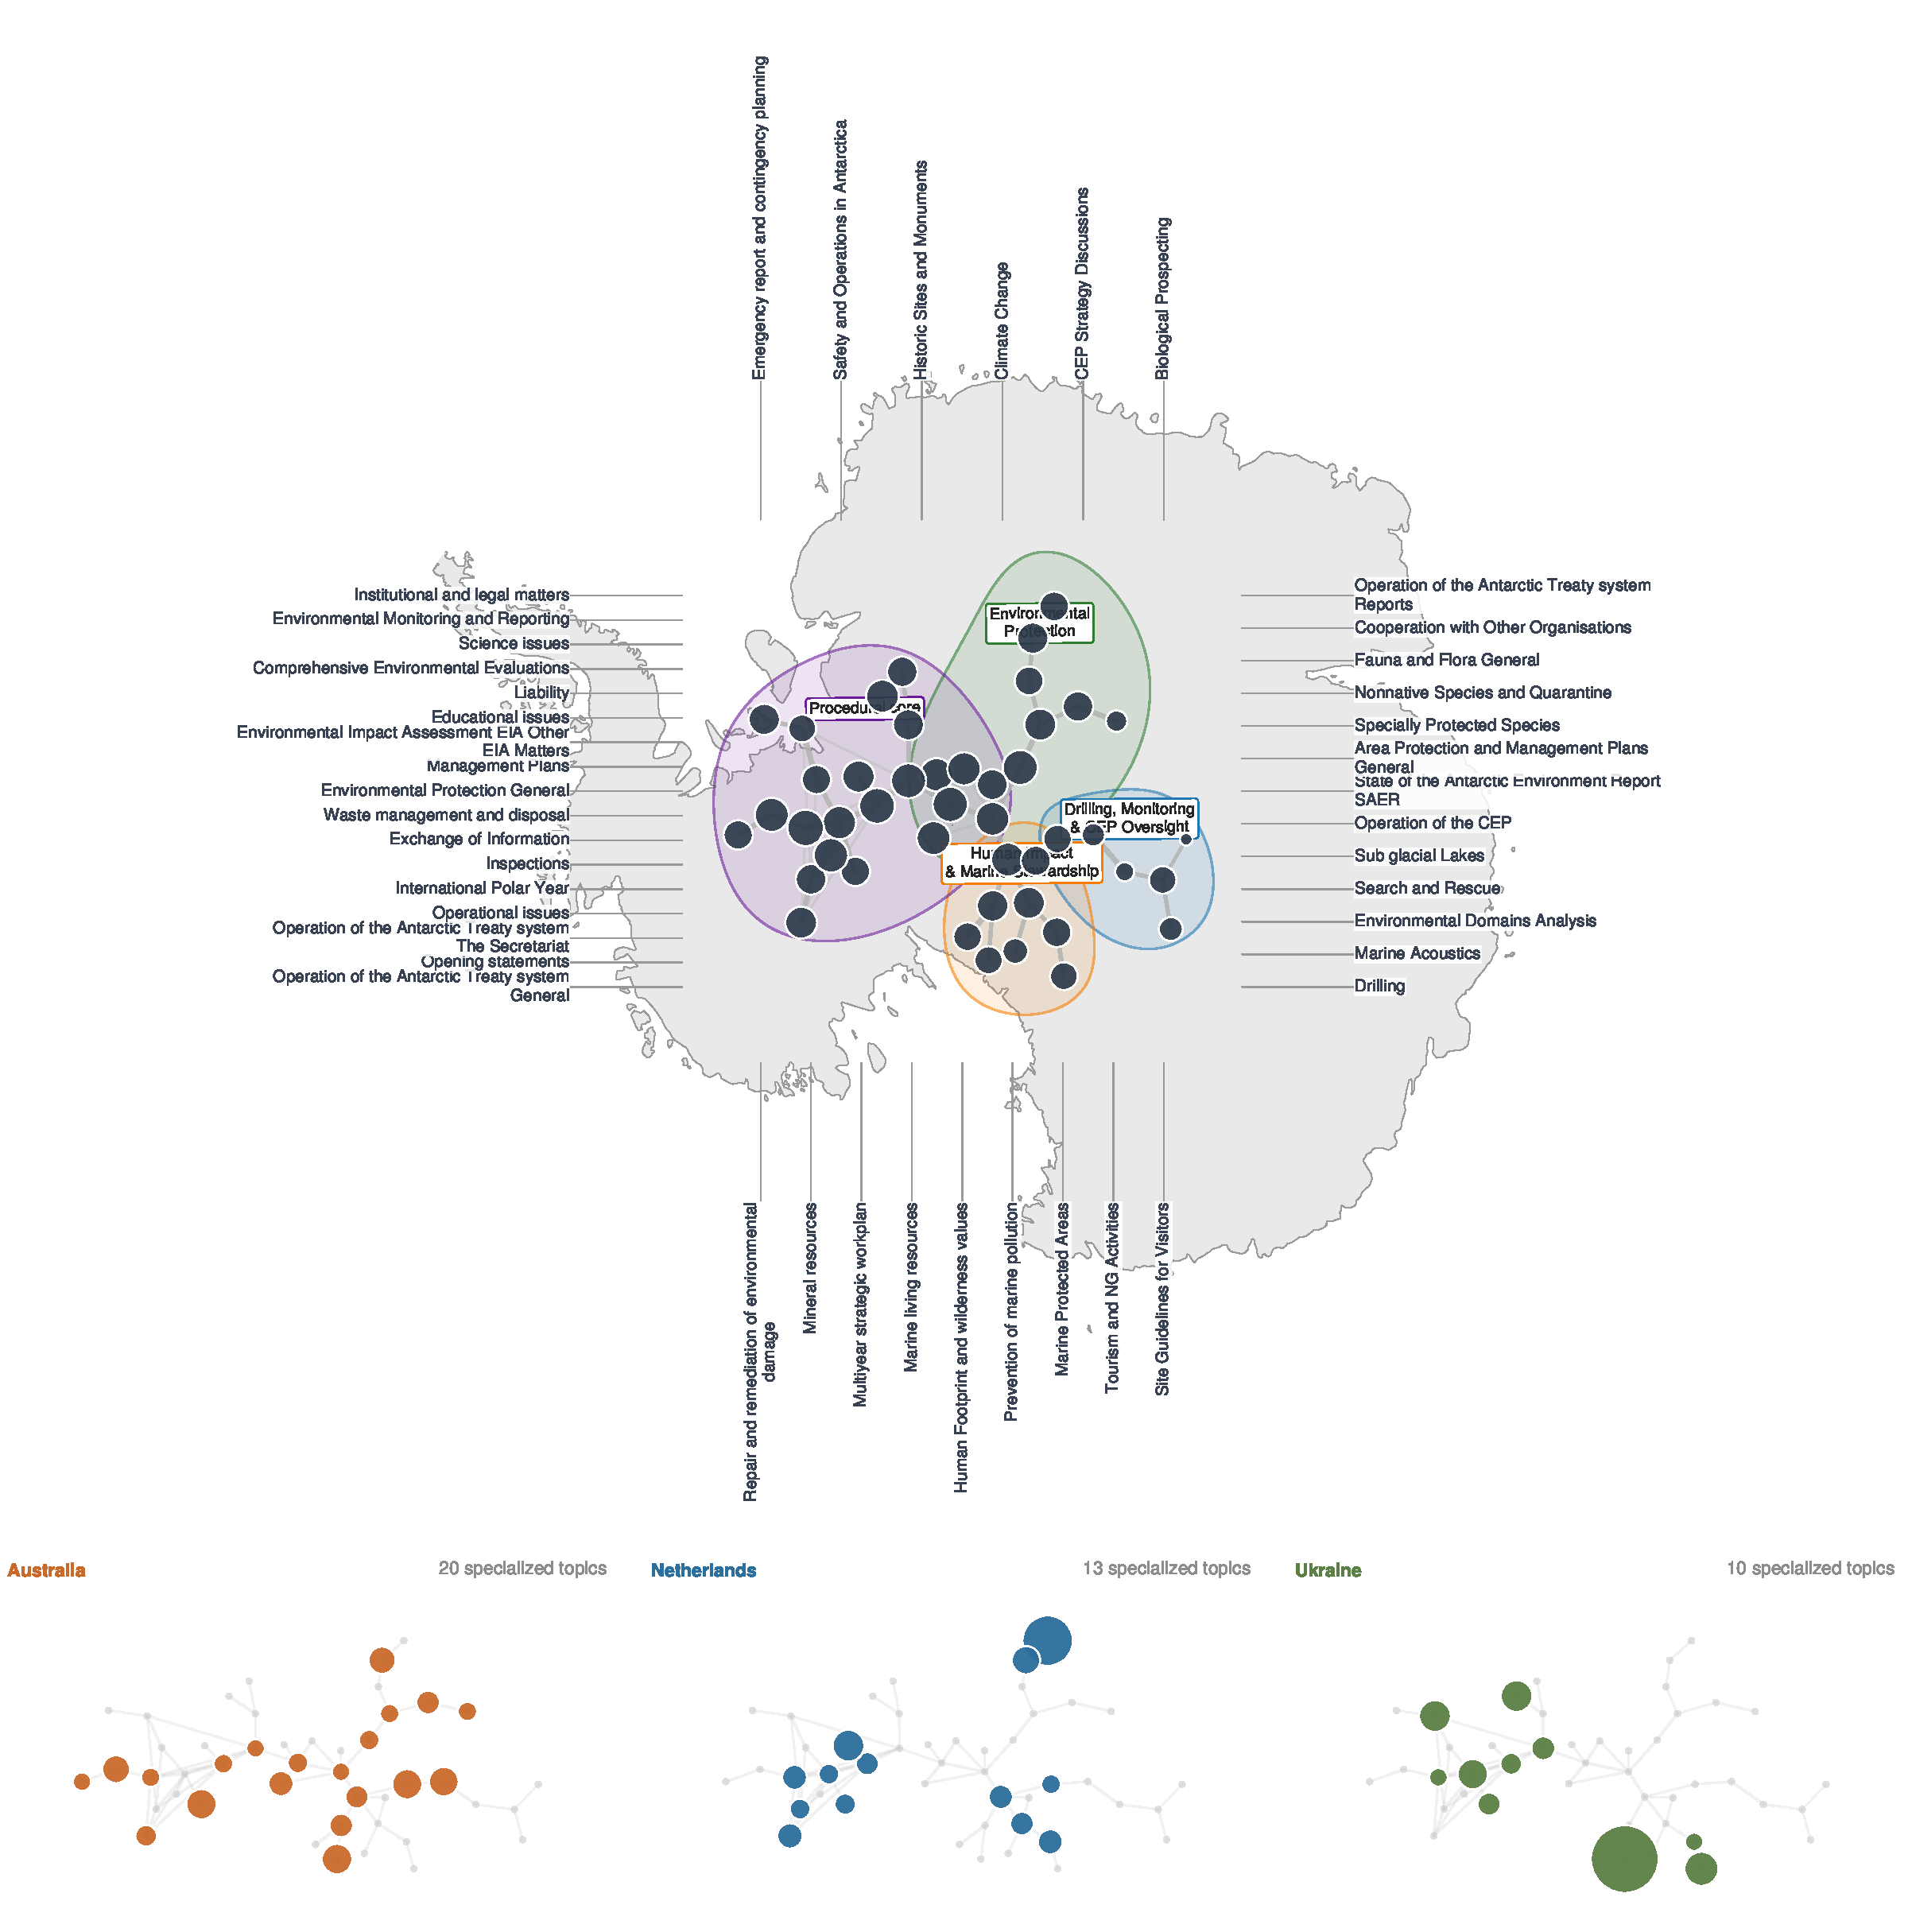
\includegraphics[width=\textwidth]{./figures/fig01_space_of_concerns_topology.pdf}
\caption{\textbf{Treaty papers form a connected concern space with permeable regions.} Two concerns are close when the same actors devote an above-average share of their papers to both. The space is drawn as a transit diagram: concerns are stations, colours identify the seven-region CPM reading, and dashed links cross between regions. Larger stations are more strongly connected, outer rings mark concerns that bridge several regions, and diamonds mark the five concerns whose bootstrap assignment favours another region. The displayed connections combine bootstrap-supported relations with the minimum scaffold needed to keep all 45 concerns visible in one network. Horizontal, vertical, and diagonal routes are a visual simplification; their direction and length carry no substantive meaning. Supplementary Information \cref{fig:cpm-partition-comparison,fig:cpm-uncertainty} reports the partition comparison and uncertainty.}
\label{fig:the_space_of_concerns}
\end{figure*}

\section{Results}
\subsection{Treaty papers form an uneven concern space}
While the annexes describe the founding tenants of the ATS, the space of concerns provide insights in how attention fills those tenants, create concerns and most importantly connect them (\cref{fig:the_space_of_concerns}). We find that the space is not easily divided into distinct blocs, rather a patchwork exists in which concerns are weakly modular. These blocs can be read as distinct branches of Antarctic governance. For example, we can identify a large bloc of mostly procedural operations internal to the maintance and management of the ATS (blue). This bloc is connected through inspections with a bloc focused environmental management (gray blue) and a bloc focused on resource management (green).

A seven-region CPM reading separates a procedural and scientific core and environmental management from access, tourism and safety; resources and planning; cooperation and reporting; environmental domains and reporting; and the smaller pairing of marine acoustics with sub-glacial lakes. Yet ties cross these regions throughout the map, and five boundary concerns are assigned more often to another region when actors are resampled. The regions are therefore guides to locally dense parts of a connected agenda, not fixed regimes. A concern's significance depends not only on how much attention it receives, but also on where it sits relative to the rest of the agenda.

The links between these regions make the overlap concrete. Inspections connects the procedural center to environmental management and resource planning. CEP Strategy Discussions connects that center to environmental domains and reporting, while the State of the Antarctic Environment Report and the multiyear strategic workplan join those reporting concerns to planning. Environmental Domains Analysis then continues toward marine acoustics and sub-glacial lakes. These are cross-region junctions in the displayed backbone, not evidence that one concern causes movement into another.

Pairwise proximity spans the full observed range. The strongest relation joins Marine living resources to Mineral resources ($\phi=0.667$), followed by Management Plans with Repair and remediation and Area Protection with Management Plans (both $\phi=0.625$). At the other end, Environmental Domains Analysis and Opening statements have only a weak positive relation ($\phi=0.036$), while 34 concern pairs have zero proximity because no actor specializes in both. These absences concentrate around SAER, Environmental Domains Analysis, and Sub-glacial Lakes. The agenda is therefore connected overall but highly uneven in how concerns share documentary constituencies.

The numerical results support this reading. At $\gamma=0.273$, mean proximity is $0.362$ within the seven CPM regions and $0.198$ between them, and the same partition persists from $\gamma=0.258$ to $0.291$ \cite{Traag2019}. The two distributions nevertheless overlap: cross-region proximity reaches $0.500$, while all 34 zero-proximity pairs fall across region boundaries. A coarser four-region reading preserves most of the same organization, with 43 of 45 concerns remaining within a corresponding broader region. Actor resampling shows where the boundaries soften. Mean within-region co-assignment ranges from $0.40$ to $0.79$, and the broad environmental regions often subdivide. Supplementary Information \cref{sec:cpm-reading,fig:cpm-partition-comparison,fig:cpm-uncertainty} reports the construction and uncertainty.

Treating concerns separately misses the system they form together. The space of concerns instead treats the ATS agenda as an interconnected network, in which an edge is stronger when specialization in one concern more consistently accompanies specialization in another after accounting for how widely each is held. This network is related to, but not recoverable from, marginal counts. Paper volume reconstructs only $10.7\%$ of pairwise proximity when relations involving each concern are predicted from models fitted without that concern. The number of specializing actors reconstructs $34.1\%$, and adding paper volume leaves that result unchanged. Across 1,000 actor bootstraps, paper volume adds a median of only $0.5$ percentage points after specialization prevalence is known. Counts therefore show where documentary attention accumulates whereas proximity shows how that attention is organized across actor portfolios (Supplementary Information \cref{sec:counts-versus-relations,tab:count-reconstruction}).

\begin{figure*}[!t]
 \centering
 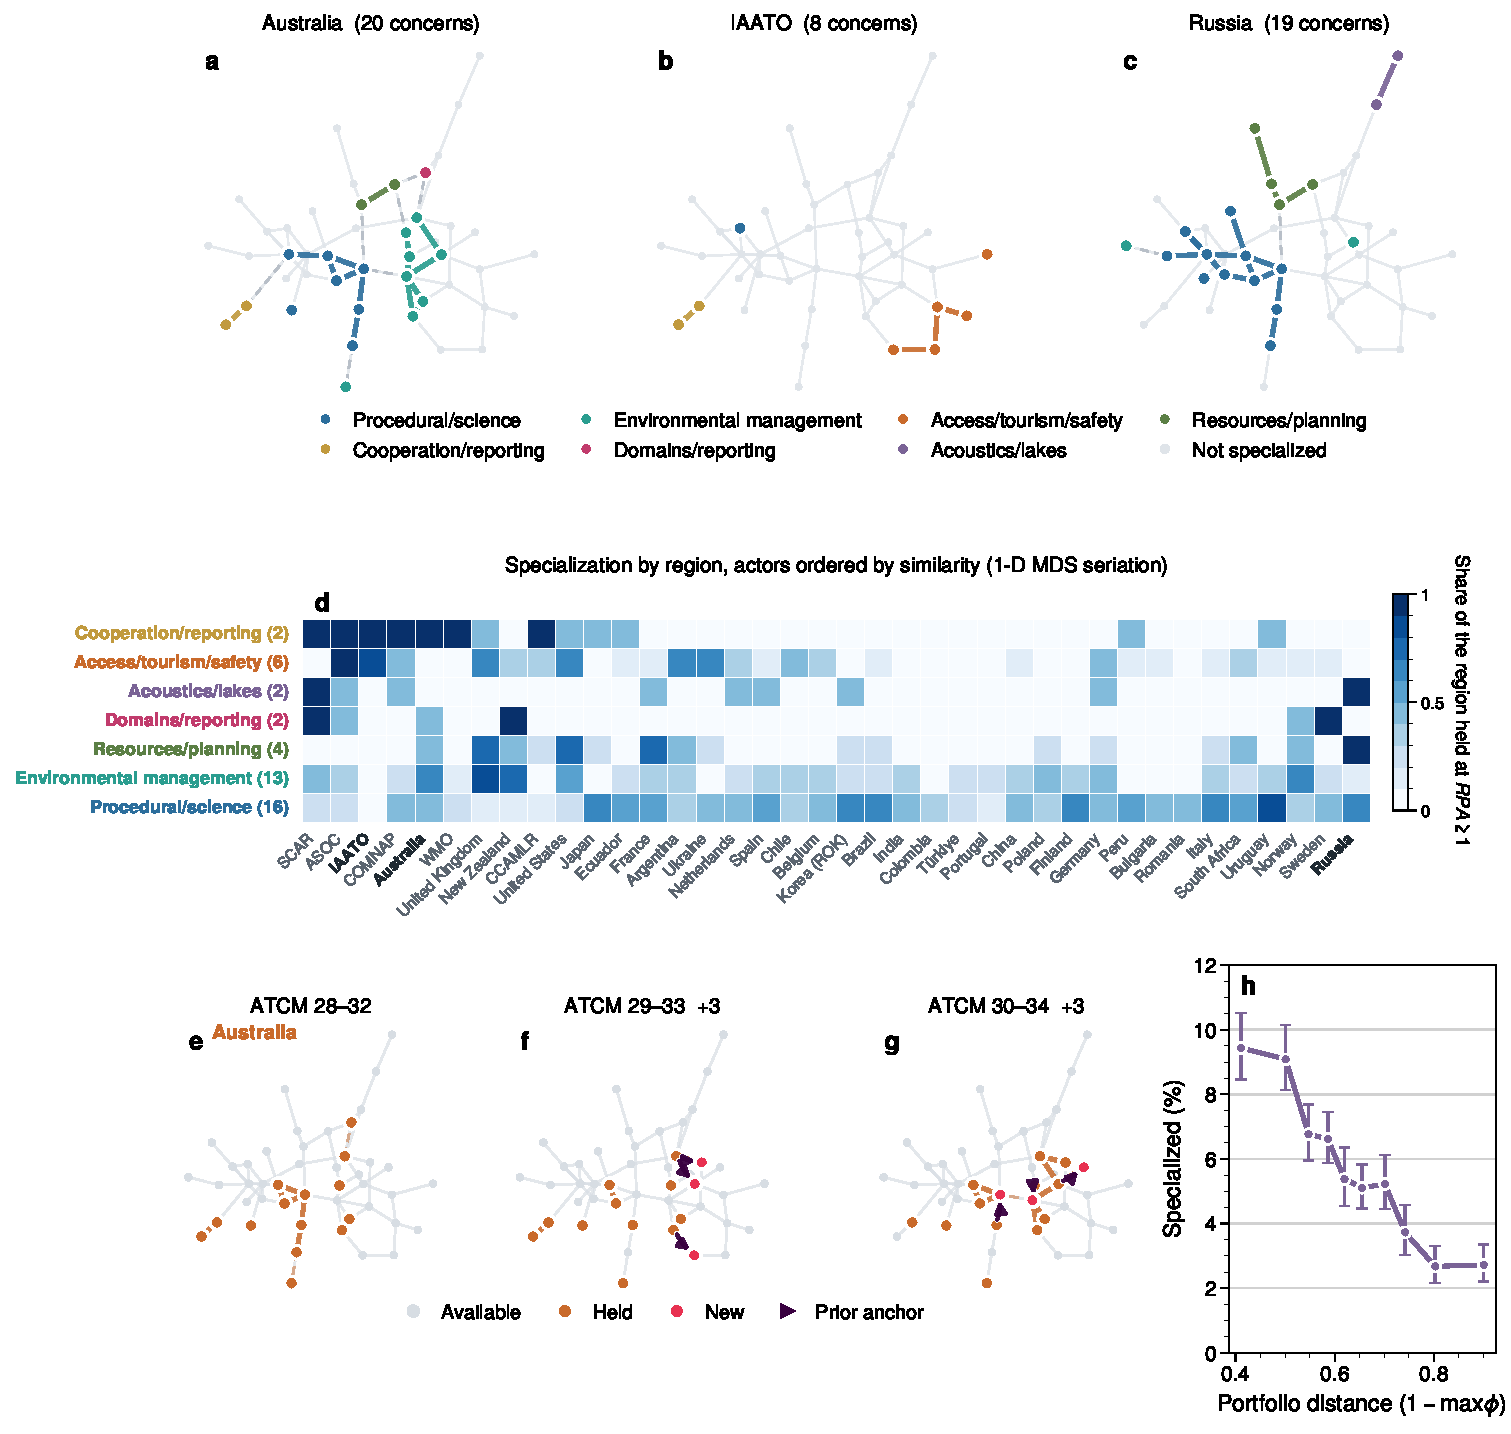
\includegraphics[width=0.95\textwidth]{figures/fig02_local_specialization.pdf}
 \caption{\textbf{New specialization is more likely near an actor's earlier portfolio.} A concern becomes specialized when its share of an actor's papers exceeds its archive-wide share. (a) Three successive Australian portfolios hold the map fixed. Pink nodes newly cross the specialization threshold, and arrows point from their nearest concern in the preceding portfolio. We show this interval because each transition adds three concerns and all six additions join the previous portfolio on the displayed backbone. (b) The observed crossing rate falls with distance, $1-\max\phi$. Points are quantile bins and bars are descriptive Wilson 95\% intervals. (c) Each observed move is compared with alternatives drawn according to prior popularity. The point shows how often actors moved to a nearer concern than popularity alone predicts; the bar is the actor-bootstrap 95\% interval. (d) Odds ratios give the change in crossing odds for a $0.1$ increase in distance. The rows report the primary model, the complete actor-history bootstrap, a first-paper outcome, and the inferred one-category analysis. Panel a illustrates movement; panels b--d test the pattern across actors and periods. Supplementary Information \cref{sec:hazard-model,sec:paired-null-robustness,fig:hazard-space-sensitivity,tab:locality_estimands} gives the full design and checks.}
 \label{fig:local-specialization}
\end{figure*}

\subsection{Earlier portfolios predict where relative attention shifts}
The upper row of \cref{fig:local-specialization} makes one sequence visible by holding the geometry fixed across ATCM 28--32, 29--33, and 30--34. Australia first adds Climate Change, Human Footprint and wilderness values, and Prevention of marine pollution next to concerns already in its portfolio. In the following window it adds Area Protection, Comprehensive Environmental Evaluations, and Inspections in the same local manner. All six additions connect to the preceding portfolio on the displayed backbone. This sequence illustrates movement but does not establish its generality.

We reconstruct portfolios in rolling five-meeting periods and mark a specialization shift when a concern's RPA crosses from below 1 to at least 1. This means that the concern's share of an actor's papers has risen above its archive-wide share; it is not necessarily the actor's first paper on the subject. We compare each crossing with concerns that already existed but were not specialized in by that actor. Distance is measured from the nearest concern in the earlier portfolio using only records that predate the shift. The model asks whether nearby concerns are more likely to cross after accounting for their prior popularity.

Across 968 actor-period comparisons and 30,957 available concerns, the observed crossing rate falls from about $9\%$ among the nearest concerns to about $3\%$ among the farthest (\cref{fig:local-specialization}a). After accounting for prior popularity, moving $0.1$ farther from the earlier portfolio is associated with $18\%$ lower odds of crossing (OR $0.817$, 95\% model-based CI $[0.783,0.853]$). Rebuilding portfolios and the map in 500 actor-history bootstrap samples attenuates the estimated effect but preserves its direction in every draw (median OR $0.869$, central 95\% $[0.820,0.918]$; \cref{fig:local-specialization}c). Actors moved to a nearer concern than expected from prior popularity in $62.5\%$ of comparisons (95\% actor-bootstrap interval $[58.9,66.5]\%$; \cref{fig:local-specialization}b). Both tests exclude concerns that had not appeared before the transition. A first-paper outcome and a one-category-per-paper construction give similar estimates. The association also remains in disjoint five-meeting blocks, although it is weaker (OR $0.904$, $[0.855,0.957]$; Supplementary Information \cref{sec:hazard-model,sec:paired-null-robustness,fig:hazard-space-sensitivity,tab:locality_estimands}). Stable mandates, expertise, resources, and institutional learning could all produce the pattern; the design does not separate them.

Local shifts do not mean permanent specialization. Recorded duration falls sharply and depends on how temporary gaps are treated (Supplementary Information \cref{sec:retention-method,fig:retention-curves}). Australia, the Netherlands, and Ukraine also move across the continuous concern axis rather than remaining fixed (Supplementary Information \cref{fig:actor-continuous-trajectories}). The trajectories illustrate movement; the model and matched comparison establish the general local pattern. Counts show how much documentary attention a concern receives. The space shows which concerns repeatedly occupy the same actors' portfolios. This actor-level result does not show what the ATCM adopts. We next aggregate attention across actors and ask whether its meeting-level distribution helps forecast formal output.

\begin{figure*}[!t]
 \centering
 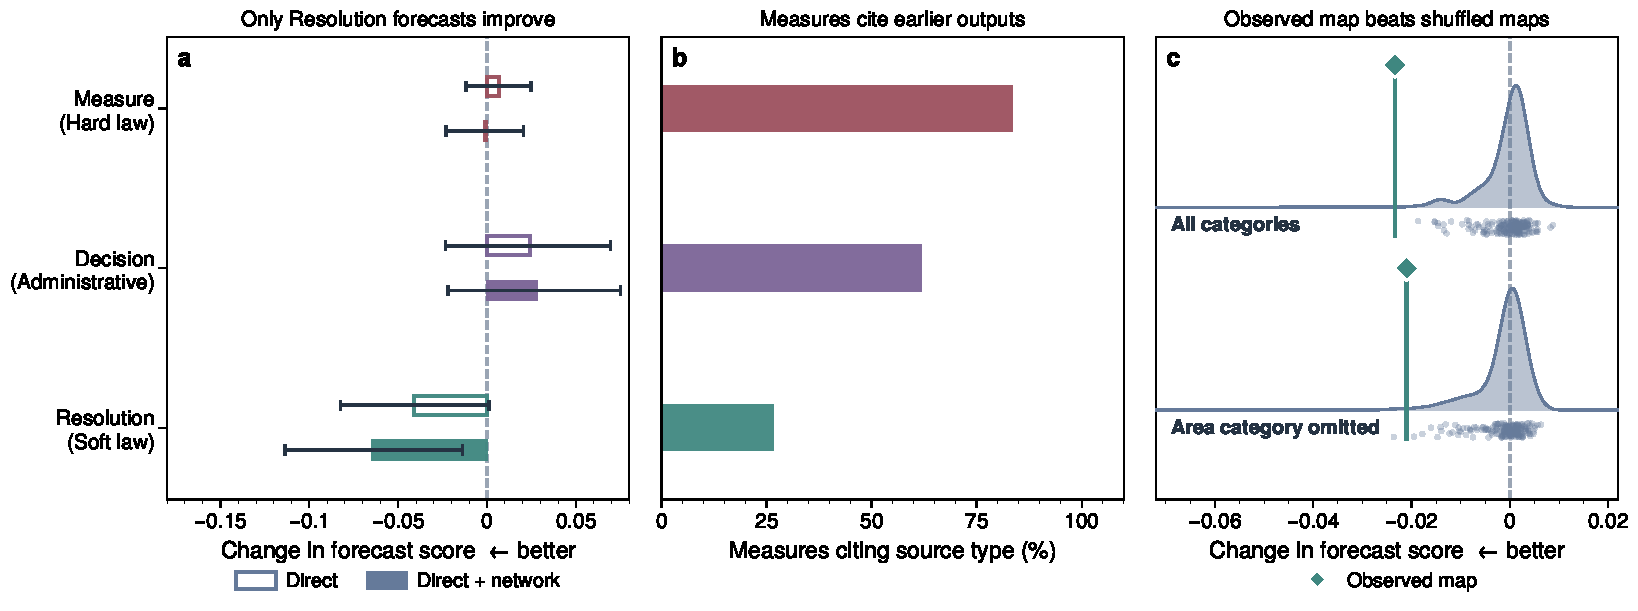
\includegraphics[width=\textwidth]{figures/fig03_attention_to_formal_tracks.pdf}
\caption{\textbf{Attention improves Resolution forecasts, while Measures draw on earlier formal outputs.} (a) Change in rolling-origin forecast score after adding direct attention or direct plus network-weighted attention to output history. Lower scores are better. Whiskers are meeting-bootstrap 95\% intervals. (b) Share of 277 Measures whose adopted body text cites each earlier output type. The rows share the labels in panel a and can overlap. (c) Resolution forecast changes for the observed map (diamonds) and 200 shuffled maps (points). The observed map beats all shuffles with every category ($p=0.005$) and 199 of 200 when Area protection and management is omitted ($p=0.010$). Citations record formal reference, not causation or implementation. Supplementary Information \cref{sec:prospective-output-forecast,sec:formal-inheritance-audit,sec:forecast-results,sec:formal-inheritance-results} gives the full design.}
 \label{fig:selective-translation}
\end{figure*}

\subsection{Attention forecasts Resolutions; Measures show formal inheritance}
We next ask whether documentary attention improves forecasts of adopted output. The inventory contains all 584 Measures, Decisions, and Resolutions adopted at regular ATCMs from 1995 through 2025: 277 Measures, 135 Decisions, and 172 Resolutions. The instrument register uses 15 broad categories, while the paper record uses 45 finer concerns. We aggregate every paper concern into one output-category family before comparing the records. A paper keeps total weight one, with its fine-category weights summed within families. Sixty outputs have more than one official category; their weight is divided equally (Supplementary Information \cref{sec:outcome-positioning}).

We first selected forecast settings from pooled outputs at ATCMs 25--28. The selected benchmark uses output from the preceding five meetings. The direct-attention model adds paper volume and the number of distinct submitters in the focal category during the immediately preceding and current meeting. We froze these settings before evaluating Measures, Decisions, and Resolutions at ATCMs 29--47. A third model adds current papers in all 14 non-focal categories, weighted by a concern map built before the meeting. Papers submitted for the focal ATCM are known before its outputs are adopted, so this is a pre-adoption forecast rather than a long-range prediction.

The combined attention model improves the Resolution forecast (\cref{fig:selective-translation}a). Relative to output history alone, it lowers the mean allocation log score by $0.065$ (95\% meeting-bootstrap interval $[-0.114,-0.014]$) and improves 15 of 19 rolling-origin test meetings. Direct attention accounts for a mean change of $-0.041$ ($[-0.082,0.001]$); network attention changes the direct model by a further $-0.023$ ($[-0.050,0.002]$). These component intervals cross zero, but their combined change does not. The same combined model does not improve the output-history forecast for Measures ($-0.001$, $[-0.023,0.020]$) or Decisions ($0.028$, $[-0.022,0.075]$). The Resolution gain is $0.063$ larger than the Measure gain ($[-0.112,-0.012]$) and $0.092$ larger than the Decision gain ($[-0.159,-0.022]$).

The geometry itself carries information. Adding an unweighted count of all papers outside the focal category changes the direct Resolution model by $0.001$ ($[-0.001,0.003]$), whereas the network-weighted count changes it by $-0.023$. In a stricter null, we coherently reassign both endpoints of every pre-meeting map, recompute network attention, and refit the forecasts. The observed geometry beats all 200 shuffled maps (lower-tail $p=0.005$; \cref{fig:selective-translation}c). It beats 199 of 200 when Area protection and management is omitted from the scored categories ($p=0.010$). The mean network gain remains negative when each category is omitted from scoring in turn and under all tested history windows, regularization values, and projections through the original 45-concern space (Supplementary Information \cref{sec:forecast-results}). Generic paper volume does not reproduce this pattern. The combined improvement is also similar below and above median category entropy ($-0.073$ and $-0.055$), so it is not confined to meetings with especially broad Resolution agendas. This comparison is descriptive.

Measures show a different association. Of the 277 Measures, 266 include Area protection and management among their official categories, 230 concern a management plan, and 211 concern a revised management plan. Earlier Measures alone forecast their category distribution better than earlier Decisions and Resolutions or attention without Measure history. Their adopted body text also refers back to established formal work. In total, 245 Measures cite at least one earlier Measure, Decision, or Resolution in the post-1995 inventory. Earlier Measures are cited by 231 later Measures, Decisions by 171, and Resolutions by 73 (\cref{fig:selective-translation}b). These rows overlap. The Decision links draw on only eight distinct Decisions, and the Resolution links on nine of the 172 Resolutions. Measures are therefore concentrated in recurring work and usually cite earlier outputs. The allocation design cannot tell whether current documentary attention also contributes.

Resolutions can still provide a bridge, but not a general escalator. Eighty of the 81 exact Resolution-to-Measure citations occur in protected-area or heritage administration. The only link outside those domains runs from Resolution 4 (2007) on ship-based tourism to Measure 15 (2009) on passenger-vessel landings. Exact citations are a conservative record of formal inheritance, not a complete policy lineage. We use them to identify cases for closer study rather than treating a shared category as proof of a link (Supplementary Information \cref{sec:formal-inheritance-results}).

\section{Discussion}
The Antarctic record separates two patterns in institutional work. Actors usually shift disproportionate attention toward concerns close to their earlier portfolios. Direct and network-weighted attention together improve forecasts of where the ATCM adopts non-binding Resolutions. Measures look different: they cluster in recurring area-management work and refer heavily to earlier formal outputs. Documentary attention therefore has different forecasting value across the three forms of output.

This distinction adds a relational layer to agenda measurement. Counts show how much attention a concern receives. The concern space shows which concerns repeatedly occupy the same actors' portfolios and narrows the set of likely next specializations. Direct papers and network-weighted attention also contain information about the category distribution of Resolutions that is absent from earlier output alone. An unweighted count of all papers outside the category does not provide the same gain, and shuffled maps lose it. The relation depends on the observed geometry rather than paper volume in general.

Resolutions are the broadest of the three output types in this record. They are non-binding and can state recommendations, principles, or shared positions without the approval process required for a Measure. Across this wider category distribution, concern-network attention improves the forecast. The gain is comparable in lower- and higher-entropy Resolution meetings, so it is not carried only by meetings with unusually broad output. Resolutions span a wider adopted agenda than Measures or Decisions.

Measures show continuity of a different kind. Prior Measures forecast them far better than prior Decisions and Resolutions or current attention alone. Their adopted body texts reinforce that result: 231 of 277 cite an earlier Measure. Much of this continuity comes from protected-area plans that are revised through repeated Measures. Exact citations establish formal reference, and they show that Measures often draw on an existing formal record.

Soft law appears in some of that inherited record, but explicit Resolution-to-Measure links are rare. Only nine of 172 Resolutions are cited by a later Measure, and almost every citation concerns protected areas or heritage. The tourism sequence is the sole exception. Resolution 4 (2007) addressed ship-based tourism, and the ATCM later adopted comparable passenger-vessel landing limits in Measure 15 (2009). Liability shows why exact citations are still a lower bound. Decision 3 (1998) moved further negotiation of a liability annex to ATCM Working Group I, Resolution 5 (1999) requested practical and scientific input, Decision 3 (2001) advanced a draft, Measure 1 (2005) adopted Annex VI, and Decision 1 (2005) established annual review of progress towards its becoming effective. The final Measure does not cite the 1999 Resolution. Annex VI and Measure 15 (2009) also remain not effective in the official register. These cases show formal development, not completed conversion into binding law or implementation \cite{ATCMAnnexVI2005,ATCMMeasure152009}.

Institutional adaptation therefore has distinct observable stages. The concern map locates new issues relative to work that actors already sustain. The Resolution forecast tests whether the distribution of attention helps locate formal but non-binding output. The Measure audit records continuity with earlier formal work. Entry into force, implementation, and environmental outcomes extend the assessment beyond adoption.

The evidence comes from the public documentary record. Actor positions describe participation rather than bargaining power, and only Consultative Parties take decisions. The nodes follow the database taxonomy, while the 15 output families form an analytic hierarchy. RPA combines choice with mandate, expertise, reporting duties, and resources, and the archive excludes informal bargaining and Conference Room Papers. Position before 1991 also did not identify responses to the Madrid Protocol reorientation, placing major institutional change outside the routine local pattern (Supplementary Information \cref{sec:madrid-shock}). These boundaries matter most when transferring the design to institutions without repeated actors, stable categories, public inputs, and observable outputs.

The concern space turns submitted papers into more than a count. It forecasts where actors shift relative attention and helps locate soft-law output. Measures follow a narrower formal record. For document-rich consensus institutions, the lesson is simple: map attention early, but assess binding adaptation separately through legal status, implementation, and environmental outcomes.

\subsection*{Author Contributions}
\textbf{Casper van Elteren:} conceptualization; methodology; software; formal analysis; investigation; data curation; visualization; writing, original draft; writing, review and editing. \textbf{Fiona Lippert:} conceptualization; writing, review and editing. \textbf{Vítor V. Vasconcelos:} conceptualization; writing, review and editing. \textbf{Zach Carter:} writing, review and editing. \textbf{Maria Kleshnina:} supervision; funding acquisition; writing, review and editing. \textbf{Michael Bode:} writing, review and editing. All authors contributed to the final manuscript.

\subsection*{Declaration of interests}
All authors declare no competing interests.

\subsection*{Ethics declaration}
This study analyzes publicly available institutional documents and does not involve human participants, personal data, or animal research.

\subsection*{Resource availability}
\noindent\textbf{Lead contact:} Casper van Elteren (casper.vanelteren@qut.edu.au).\\
\textbf{Materials availability:} This study analyzes existing documentary records; no new materials were generated.\\
\textbf{Data and code availability:} The June 2026 analysis archive is available at Zenodo (\url{https://doi.org/10.5281/zenodo.20821775}). A self-contained review archive containing the reconstructed many-to-many paper panel, the pinned corpus of 277 official Measure body texts, the formal-output inputs, analysis scripts, and derived tables has been prepared for editorial and peer review. The same materials will be deposited as a new version of the Zenodo record before publication. Analysis scripts use Python 3.13 with NumPy, pandas, and SciPy; figures use UltraPlot \cite{vanElteren2025}. Development code is maintained at \url{https://github.com/cvanelteren/theSpaceOfConcerns}.

\subsection*{Funding}
This work was supported by the Australian Research Council Special Research Initiative Securing Antarctica's Environmental Future (SR200100005), and by an Australian Research Council DECRA Fellowship awarded to Maria Kleshnina (DE250101223).

\subsection*{Acknowledgments}
C.v.E. would like to thank Larissa Lubiana Botelho for discussions and inputs regarding the manuscript and the Antarctic Treaty System at large.

\printbibliography
\clearpage
\appendix
\setcounter{figure}{0}
\setcounter{table}{0}
\renewcommand{\thefigure}{S\arabic{figure}}
\renewcommand{\thetable}{S\arabic{table}}
\section*{Supplementary Information}
\addcontentsline{toc}{section}{Supplementary Information}

The Supplementary Information follows the order of the main claims and retains only analyses needed to define, support, or bound them.

\begin{itemize}
 \item \textbf{Data and measurement.} Archive construction, the multi-label institutional taxonomy, actor types, the concern space, a count-reconstruction test, and output positioning.
 \item \textbf{Portfolio development.} Tests of specialization shifts, duration, cohort differences, and robustness.
 \item \textbf{From attention to output.} Rolling-origin forecasts by output type, an audit of formal inheritance, pooled association checks, and the Madrid Protocol boundary test.
\end{itemize}

\section{Data and Methods}
\subsection{Data and archive coverage}
We analyze working papers and information documents submitted from 1961 to 2025. ``ATS'' refers to the broader governance system anchored in the Antarctic Treaty, but our corpus comes only from the Treaty-centered archive of Antarctic Treaty Consultative Meetings (ATCMs). The Secretariat's taxonomy also includes topics handled by the Committee for Environmental Protection because these matters reach the ATCM agenda. Meeting volume rises partly for institutional reasons: ATCMs became annual in the 1990s, and the Committee has normally met annually since 1998. Conference Room Papers are not systematically available and are excluded. The corpus therefore observes formal documentary preparation, not the informal negotiation record.

The official archive supplies thematic search categories, submitters, and document types \cite{Yaryab2024}. We retain Secretariat papers, so the Secretariat appears both as maintainer of the database categories and as one of the 66 submitting actors. Its papers enter on the same terms as those of other submitters.

We collected the data on 6 February 2026 from the ATS website (\url{https://www.ats.aq/devAS/Meetings/DocDatabase?lang=e}) with Carlo Hamalainen's antarctic-database-go collector (\url{https://github.com/carlohamalainen/antarctic-database-go}). The collector stores HTTP responses, source documents, and processing status in SQLite. These cached records permit deterministic reruns even if the website changes.

The categories are not derived from paper text. They are the harmonized cross-meeting categories under which the Secretariat-maintained database returns each paper. A paper can appear under several categories, although the returned paper payload does not itself carry a category field. The concern space therefore describes co-specialization within an institutional taxonomy, not semantic similarity. The processed many-to-many panel and reconstruction code will be included in the next Zenodo version.

We reconstructed paper--category relations from the collector's cached category-query responses, then deduplicated attachment-linked records by \texttt{paper\_id}. This produced 6,591 unique papers. We removed 18 papers (0.3\%, all after 2010) returned only under the placeholders \texttt{ALL} or \texttt{Other}, leaving 6,573 papers and 7,895 substantive paper--category relations. Of the retained papers, 5,345 have one category and 1,228 have two to five. We divide a paper with $k$ categories equally among them, so it contributes $1/k$ to each label. Papers with multiple sponsors are then expanded to one row per submitting actor; each sponsor receives the paper's same fractional category weights. The extracted and reconstructed dataset contains the following columns.

\small
\vspace{1em}
\begin{tabular}{@{}p{0.45\columnwidth} p{0.45\columnwidth}@{}}
\texttt{meeting\_year} & \texttt{paper\_id} \\
\texttt{meeting\_type} & \texttt{party\_type} \\
\texttt{meeting\_number} & \texttt{paper\_name} \\
\texttt{meeting\_name} & \texttt{paper\_number} \\
\texttt{party} & \texttt{paper\_revision} \\
\texttt{category} & \texttt{paper\_language} \\
\texttt{page\_url} & \texttt{paper\_url} \\
\texttt{page\_nr} & \texttt{exists} \\
\texttt{payload\_json} & \texttt{agendas} \\
\texttt{attachment\_id} & \texttt{parties} \\
\texttt{attachment\_name} &\texttt{attachment\_language} \\
\texttt{attachment\_url} & \texttt{attachment\_exists} \\
\vspace{1em}
\end{tabular}
The June 2026 archive is available at \url{https://doi.org/10.5281/zenodo.20821775}; the reconstructed many-to-many panel will be added in the next version.

\begin{figure*}[!htbp]
\centering
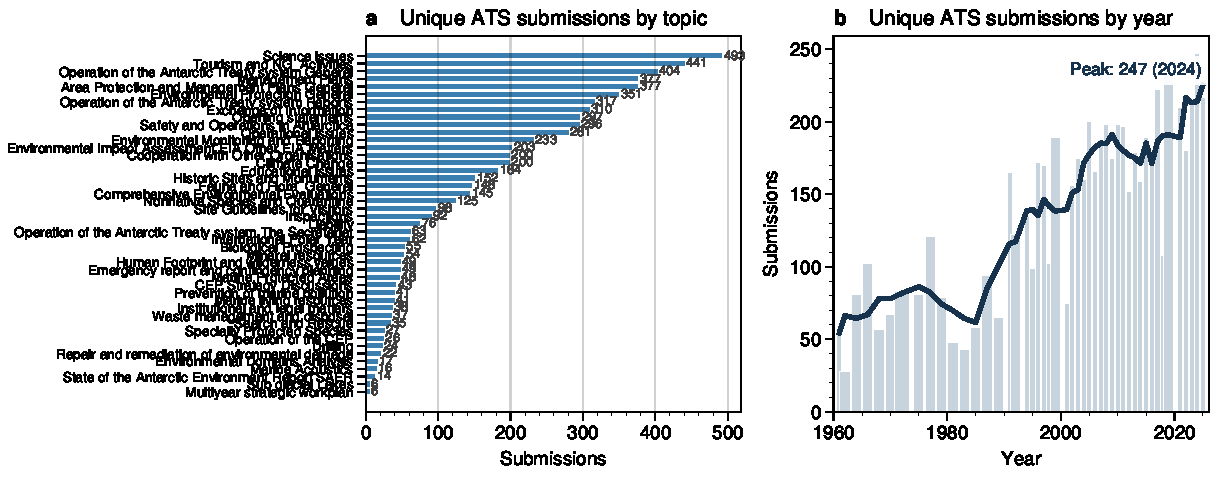
\includegraphics[width=\textwidth]{./figures/figS02_archive_coverage.pdf}
\caption{\textbf{Paper coverage expands sharply after 1990 and remains uneven across concerns.} (a) Fractional paper counts by official concern from 1961 to 2025. A paper returned under $k$ concerns contributes $1/k$ to each. (b) Unique papers submitted each year, with the centred five-year average shown as a line.}
\label{fig:topic-submission-overview}
\end{figure*}

The unit is the \emph{submitting actor}, not legal status under the Treaty. We include Consultative Parties, Non-Consultative Parties, Observers, invited Expert organizations, and the Secretariat because all appear as submitters in this documentary arena. Only Consultative Parties take decisions. The actor types are therefore not institutionally equivalent, and pooled estimates describe documentary activity rather than formal authority \cite{Sampaio2022}. Sixty-six actors appear in the corpus. The extracted field \texttt{party\_type} contains Working Paper and Information Paper codes, not Treaty status. Actor-role information is separate and can change over time. The cohort comparison retains 43 actors, while the states-only locality check retains 42 states. Conference Room Papers do not enter any analysis.

\subsection{Building the concern map}
Counts and co-specialization answer different questions. Counts show where attention is common. Co-specialization shows which concerns receive a disproportionate share of the same actors' papers. A concern pursued by nearly everyone can be prominent in counts but uninformative for co-specialization because no actor stands out. A small technical community can produce the opposite pattern. Our map measures the structure of specialization, not the overall importance of a concern.

Let $x(a,i)$ denote the fractionally counted submissions by actor $a$ on concern $i$. If paper $p$ is returned under $k_p$ substantive categories, it contributes $1/k_p$ to each; a co-sponsored paper contributes those weights to every listed submitting actor. Actors include Consultative Parties, Non-Consultative Parties, Observers, invited Expert organizations, and the ATS Secretariat whenever they appear as submitters. We define the normalized activity share
\begin{equation}\label{eq:activity_share}
\pi(a,i) = \frac{x(a,i)}{\sum_j x(a,j)},
\end{equation}

and the system-wide importance of topic $i$ as

\begin{equation}\label{eq:topic_importance}
Z_i = \frac{\sum_c x(c,i)}{\sum_{d,j} x(d,j)}.
\end{equation}

The Revealed Policy Advantage (RPA; a revealed comparative advantage (RCA)-style specialization index) is then
\begin{equation}\label{eq:rpa}
 \rho(a,i) = \frac{\pi(a,i)}{Z_i}.
\end{equation}
We call this ratio \emph{revealed policy advantage} rather than the usual \emph{revealed comparative advantage} because the units are policy concerns rather than exported products. The mathematics is unchanged, but the interpretation is narrower. Submissions have not passed a competitive market test. Actors may submit to inform, comply, signal, or seek action. RPA records the concerns receiving a disproportionate share of an actor's papers. It cannot separate intent from mandate, expertise, reporting duties, or document-production capacity, and it cannot observe priorities that produce no paper. Scientific capacity may also enter the measure because Article IX(2) ties consultative status to substantial scientific research activity. Nor do concerns have an equivalent of product complexity or economic value. Co-specialization remains useful because it records how actors allocate finite documentary effort across the agenda.

Topics are linked by proximity
\begin{equation}\label{eq:proximity}
\phi(i,j)
=
\min\!\left\{
\begin{aligned}
 &\Pr\!\bigl(\rho(a,i) \ge 1 \mid \rho(a,j) \ge 1\bigr),\\
 &\Pr\!\bigl(\rho(a,j) \ge 1 \mid \rho(a,i) \ge 1\bigr)
\end{aligned}
\right\}.
\end{equation}
with
\begin{equation}
 \Pr(\rho(a,j)\ge1 \mid \rho(a,i)\ge1) =\frac{\sum_a \mathbf{1}[\rho(a,i)\ge1 \land \rho(a,j)\ge1]}
 {\sum_a \mathbf{1}[\rho(a,i)\ge1]},
\end{equation}
yielding a weighted concern network. Conditional probability allows two uncommon concerns to be close when specialization in one reliably accompanies specialization in the other; a joint probability would shrink mechanically with rarity. Taking the lower of the two directions prevents a niche concern from appearing close to a broad concern merely because the niche usually occurs alongside it. The result is symmetric and measures mutual co-specialization. Probabilities are estimated across actors in the relevant window. With 66 actors, individual links rest on modest counts: the strongest tie, between Marine living resources and Mineral resources, rests on 6 actors. The map is therefore a coarse aggregate rather than a high-resolution estimate of every pair. We construct a pooled map and rebuild time-specific maps within each window. This adapts product-space proximity to governance concerns \cite{Hidalgo2007}.

\subsection{Can marginal counts reconstruct the concern space?}\label{sec:counts-versus-relations}
To test whether proximity is only a reformulation of prevalence, we treat each of the 990 concern pairs as one observation and use pooled $\phi(i,j)$ as the outcome. For each pair, the paper-count model contains the sum, absolute difference, and minimum of the two concerns' log-transformed marginal paper volumes. The actor-prevalence model uses the corresponding functions of the number of actors with $\mathrm{RPA}\ge1$. A combined model includes both sets. These are reconstruction diagnostics, not causal models.

We assess generalization with a leave-endpoint-out procedure. For each concern, we omit every pair containing it, fit the model to the remaining pairs, and predict the omitted relations. Each pair is predicted twice, once from a fit excluding each endpoint, and the two predictions are averaged before calculating $R^2$. We then resample the 66 complete actor histories 1,000 times and rebuild paper volume, RPA assignments, the full proximity matrix, and every model in each draw. Finally, 9,999 node-label QAP permutations randomly reassign the observed marginal attributes to concerns while leaving the proximity matrix fixed. This preserves the marginal distributions while testing whether their observed alignment with the network exceeds arbitrary assignments.

Paper volume explains $12.8\%$ of pooled proximity and $10.7\%$ when predicting relations involving a concern omitted from model fitting (\cref{tab:count-reconstruction}). Specialization prevalence explains $35.3\%$ pooled and $34.1\%$ under the same test. The combined model reaches $35.9\%$ pooled but remains at $34.1\%$ when concerns are omitted. Across actor bootstraps, the additional pooled variance explained by paper volume after actor prevalence has a median of $0.005$ and a central 95\% interval of $[0.0003,0.0173]$. All three observed pooled $R^2$ values exceed every corresponding QAP draw ($p=0.0001$). Marginal prevalence therefore aligns with the concern space, as expected for a proximity constructed from specialization, but it does not reconstruct most pairwise variation. \path{scripts/counts_vs_relations.py} reproduces the analysis.

\begin{table*}[!htbp]
\centering
\small
\caption{\textbf{Marginal counts recover only part of pairwise concern proximity.} Pooled $R^2$ measures in-sample reconstruction across 990 concern pairs. Leave-endpoint-out $R^2$ predicts links involving a concern excluded from model fitting. Bootstrap entries are medians with central 95\% intervals from 1,000 actor resamples. QAP $p$ values compare the pooled result with 9,999 random assignments of the marginal attributes.}
\label{tab:count-reconstruction}
\begin{tabular}{@{}lcccc@{}}
\hline
Model & Pooled $R^2$ & Leave-endpoint-out $R^2$ & Actor-bootstrap $R^2$ & QAP $p$ \\
\hline
Paper volume & 0.128 & 0.107 & 0.083 $[0.016,0.199]$ & 0.0001 \\
Specializing actors & 0.353 & 0.341 & 0.288 $[0.182,0.409]$ & 0.0001 \\
Both & 0.359 & 0.341 & 0.295 $[0.188,0.413]$ & 0.0001 \\
\hline
\end{tabular}
\end{table*}

\subsection{Testing whether specialization shifts toward nearby concerns}\label{sec:hazard-model}
We compare adjacent rolling five-meeting windows. A concern enters the comparison only when the actor was not already specialized in it. For actor $a$, concern $i$, and transition from $t-1$ to $t$, this condition is
\[
\text{at-risk}_{a i t}=1 \iff \rho_{a i, t-1} < 1.
\]
The binary outcome is then
\[
y_{a i t}=1 \iff \rho_{a i, t} \ge 1 \ \text{and}\ \rho_{a i, t-1} < 1.
\]
Let the previously active support be
\[
S_{a,t-1}=\{j:\rho_{aj,t-1}\ge 1\},
\]
let $A_{t-1}$ be the concerns that have appeared in the archive before the transition, and let the available set be
\[
R_{at}=\{i\in A_{t-1}:\rho_{ai,t-1}<1\},
\]
and let $m_{at}=\sum_{i\in R_{at}} y_{ait}$ denote the number of specialization crossings in an actor-period. Our main locality specification is then an actor-period conditional logit,
\begin{dmath}
\Pr(\mathbf{y}_{at}\mid m_{at}, X_{at})
\propto
\exp\!\left(
\sum_{i\in R_{at}}
y_{ait}\bigl(
\beta_d d_{a i, t-1}
\!+\!
\beta_p \mathrm{pop}_{i,t-1}
\bigr)
\right),
\end{dmath}
where
\[
d_{a i, t-1}=1-\max_{j\in S_{a,t-1}}\phi(i,j)
\]
is the distance from candidate concern $i$ to the actor's earlier portfolio and $\mathrm{pop}_{i,t-1}$ is its prior popularity (the share of actors with $\mathrm{RPA} \ge 1$). The model holds constant how many concerns cross the threshold in that period. It therefore compares which available concerns cross for the same actor at the same time, rather than comparing actors with different general rates of expansion. Periods in which an actor has no earlier portfolio or no threshold crossing do not enter the model. Differences in the number of concerns already held are constant within each actor-period comparison. The map, portfolio membership, and crossings all use $\mathrm{RPA}\ge1$.

The prospective rule leaves 968 actor-period comparisons and 30,957 available concerns. The distance coefficient is $-2.02$ (SE $0.22$), or an odds ratio of $0.817$ per $+0.1$ distance (95\% model-based CI $[0.783,0.853]$). The rule is primary because neither the map nor the choice set uses information first observed during the transition. A second outcome requires no paper on the concern in the earlier window and at least one in the next. It gives an odds ratio of $0.874$ ($[0.834,0.916]$), showing that the local association is not only a consequence of the relative specialization threshold. \path{scripts/compare_major_results_category_treatments.py} reproduces both estimates.

The example trajectories in Supplementary \cref{fig:actor-continuous-trajectories} are constructed on a continuous axis. We compute RPA in rolling five-meeting windows and locate each actor on the horizontal axis of the fixed pooled map as the RPA-weighted mean of its concern coordinates. Windows with fewer than three concerns at $\mathrm{RPA}\ge1$ are omitted. Australia connects this continuous summary to the snapshots in \cref{fig:local-specialization}, while the Netherlands and Ukraine provide two further examples. The trajectories illustrate movement rather than testing locality. \texttt{figS22\_actor\_trajectories.py} reproduces the figure.

\begin{figure*}[!htbp]
\centering
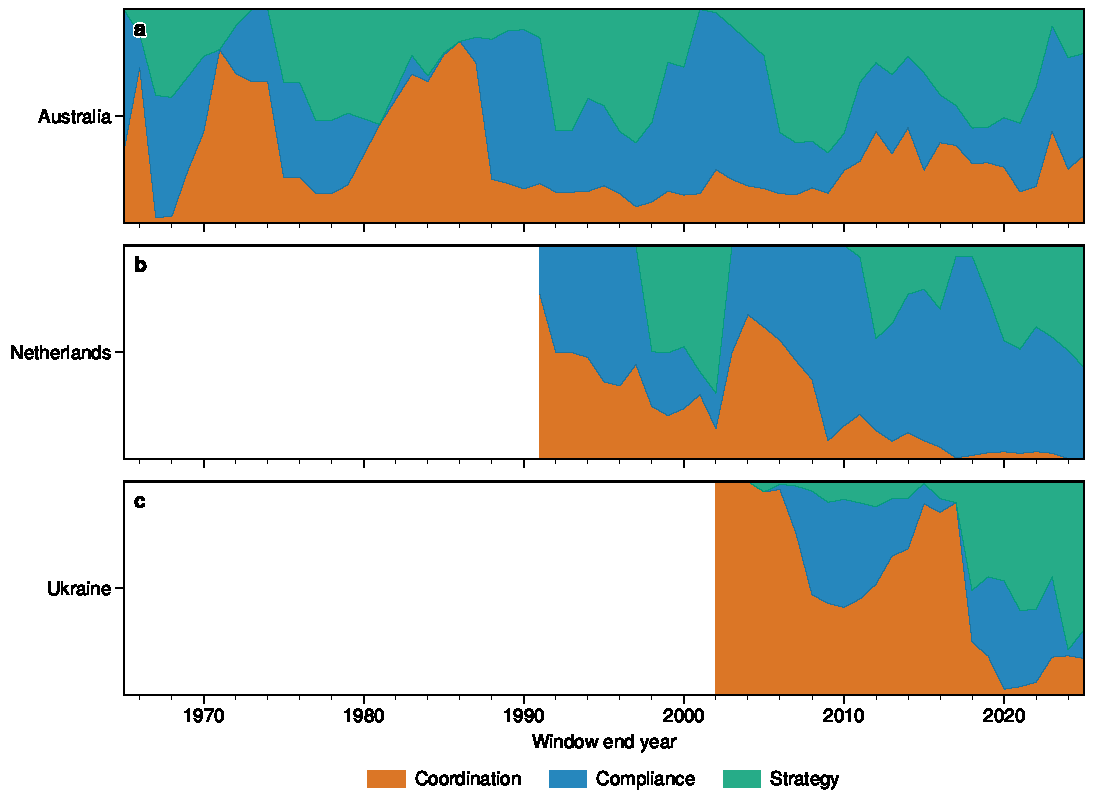
\includegraphics[width=0.92\textwidth]{./figures/figS22_actor_trajectories.pdf}
\caption{\textbf{Actor portfolios move across the concern map.} Lines show the RPA-weighted mean position of each actor's concerns along the map's horizontal axis in rolling five-meeting windows. Windows with fewer than three specialized concerns are omitted. Australia uses the same colour as in \cref{fig:local-specialization}; the Netherlands and Ukraine use the shared actor palette. These three trajectories illustrate movement. \Cref{fig:local-specialization} provides the population-level test.}
\label{fig:actor-continuous-trajectories}
\end{figure*}

Because the rolling windows overlap, successive choice sets for the same actor are not statistically independent. We therefore resample complete actor histories and rebuild portfolios, historical availability, the cumulative map, and the choice model over 500 bootstrap replicates. We also use disjoint five-meeting blocks and restrict the panel to states. The blocks reduce rolling-window overlap, but successive actor transitions still share their middle block and use nested cumulative maps; the actor-history bootstrap is the dependence-aware inference. The association remains negative in both checks; with disjoint blocks, the odds ratio is $0.904$ ($[0.855,0.957]$). These checks are reported in \cref{tab:locality_estimands}. The result is also stable across the full-archive, previous-window, and earlier-record maps while holding the prospective choice set fixed (\cref{fig:hazard-space-sensitivity}). The primary distance is raw $1-\phi$, which is bounded and directly interpretable; $-\log\phi$ is unstable when two concerns have zero proximity. \path{scripts/bootstrap_fractional_locality.py} and \path{scripts/hazard_robustness_dependence.py} reproduce the dependence checks.

\subsection{How long specialization lasts}\label{sec:retention-method}
We estimate specialization spells on 1-year windows. A spell begins when an actor first crosses $\mathrm{RPA}\ge1$ for a concern and is followed until inactivity exceeds an allowed gap of one to five consecutive years; spells still active at the end of 2025 are right-censored. Kaplan--Meier curves are computed separately for each gap definition. Because failure cannot be declared during the allowed gap itself, every curve is mechanically equal to one over that initial interval. \Cref{fig:retention-curves} reports all five definitions on the unshifted time-since-entry scale. The analysis does not distinguish a concern-specific lapse from years in which the actor submits nothing, so it is a descriptive sensitivity analysis rather than evidence of a retention mechanism.

\begin{figure}[!htbp]
\centering
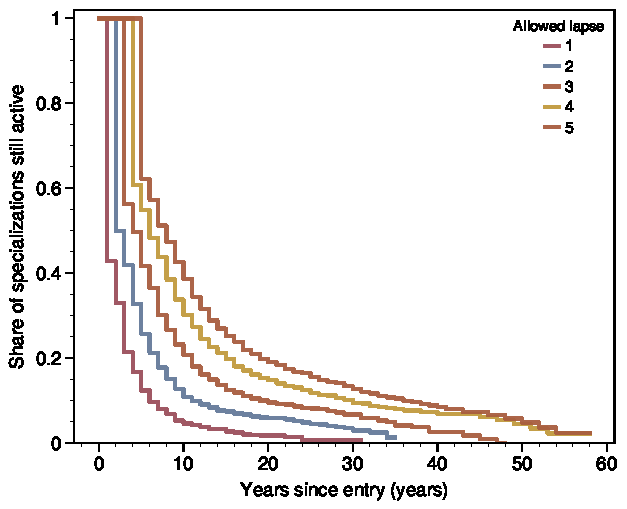
\includegraphics[width=0.46\textwidth]{./figures/figS_retention_after_entry.pdf}
\caption{\textbf{Specialization decays under every lapse rule.} Curves show the share of specialization spells still active after entry when failure requires more than one to five inactive years. The five-year curve is therefore fixed at one through year five. At ten years, survival ranges from $0.05$ to $0.42$. By twenty years every estimate is below $0.20$. Spells active in 2025 are censored. The record cannot separate a concern-specific lapse from years with no submission by the actor.}
\label{fig:retention-curves}
\end{figure}

\subsection{A retrospective comparison at the same career stage}\label{sec:cohort-method}
The cohort analysis in \cref{sec:secondary-structure-results} compares the concerns in each actor's opening portfolio with concerns appearing during the same career stage. It scores holder breadth and nearby relations using the pooled full-record map, so this is a retrospective description rather than a reconstruction of what actors could know at the time.

An actor is eligible if at least $\mathrm{WIN}=15$ years separate its first and last appearance in the archive; the requirement excludes members joining after 2010 by construction, since their record cannot yet span the window. Its \emph{opening window} runs from its first recorded year to that year plus $\mathrm{WIN}-1$. Within that window we rebuild the actor--concern interaction matrix from the submissions falling inside it, compute RPA exactly as for the pooled space, and treat a concern as held when $\mathrm{RPA}\ge 1$. Actors holding fewer than three specialized concerns in their own opening window are dropped to avoid estimating opening position from one or two concerns; this leaves 14 actors joining 1961--80, 12 joining 1981--90, and 17 joining 1991--2010.

The comparison asks whether cohort members specialized in concerns whose full-record holders covered more or fewer concerns than expected, and whether those concerns have more or fewer nearby neighbours in the pooled map. The benchmark weights concerns by their share of recorded specialization during each actor's opening window. The 1991--2010 cohort sits at $0.929$ of this benchmark for holders' full-record portfolio size (95\% actor-bootstrap interval $[0.889,0.966]$) and $0.883$ for pooled-map neighbours ($[0.798,0.974]$). The two earlier cohorts sit near parity on both measures. Each of 400 bootstrap replicates resamples the 66 actors and rebuilds opening portfolios and availability weights while retaining the pooled concern scores. \path{scripts/cohort_partition_free.py} reproduces the comparison.

\begin{table*}[!htbp]
\centering
\scriptsize
\caption{\textbf{Later entrants begin from narrower positions in the pooled map.} Ratios compare each cohort's opening portfolios with concerns appearing during the same first 15 years of activity. A value of 1 marks the career-stage benchmark. Scores for holder breadth and nearby concerns come from the pooled full-record map, so the comparison is retrospective. Intervals are actor-bootstrap 95\% intervals from 400 resamples. $n$ counts actors with a 15-year record and at least three specialized concerns.}
\label{tab:cohort-ratios}
\begin{tabular}{@{}llrrr@{}}
\hline
\textbf{Cohort} & \textbf{Scale} & \textbf{Ratio} & \textbf{95\% CI} & \textbf{$n$} \\
\hline
1961--80 & Holders' average portfolio size & 1.00 & [0.978, 1.016] & 14 \\
1961--80 & Nearby concerns & 0.99 & [0.962, 1.021] & 14 \\
1981--90 & Holders' average portfolio size & 0.98 & [0.952, 1.012] & 12 \\
1981--90 & Nearby concerns & 1.04 & [0.975, 1.133] & 12 \\
1991--2010 & Holders' average portfolio size & 0.93 & [0.889, 0.966] & 17 \\
1991--2010 & Nearby concerns & 0.88 & [0.798, 0.974] & 17 \\
\hline
\end{tabular}
\end{table*}

\subsection{Checks on local specialization}\label{sec:substantive-sensitivity}
This subsection tests whether local specialization depends on the temporal construction of the space, the threshold-crossing definition, self-contribution to the proximity matrix, or full rather than fractional credit for co-sponsored papers. A separate subsection below asks whether the recovered space is dominated by a small number of actors.

We first change how the concern map is built while keeping the prospective choice set fixed. \Cref{fig:hazard-space-sensitivity} uses the full archive, only the previous window, or all records available before the shift. In each case, distance is $d=1-\max\phi$. Moving $0.1$ farther gives odds ratios of $0.67$, $0.78$, and $0.82$, respectively. Prior concern popularity enters each model, so the distance result is not simply a preference for popular concerns. The earlier-record map is primary because it uses no later co-specialization. We retain raw $1-\phi$ because it is bounded; taking its logarithm is unstable when two concerns have zero proximity.

\begin{figure*}
 \centering
 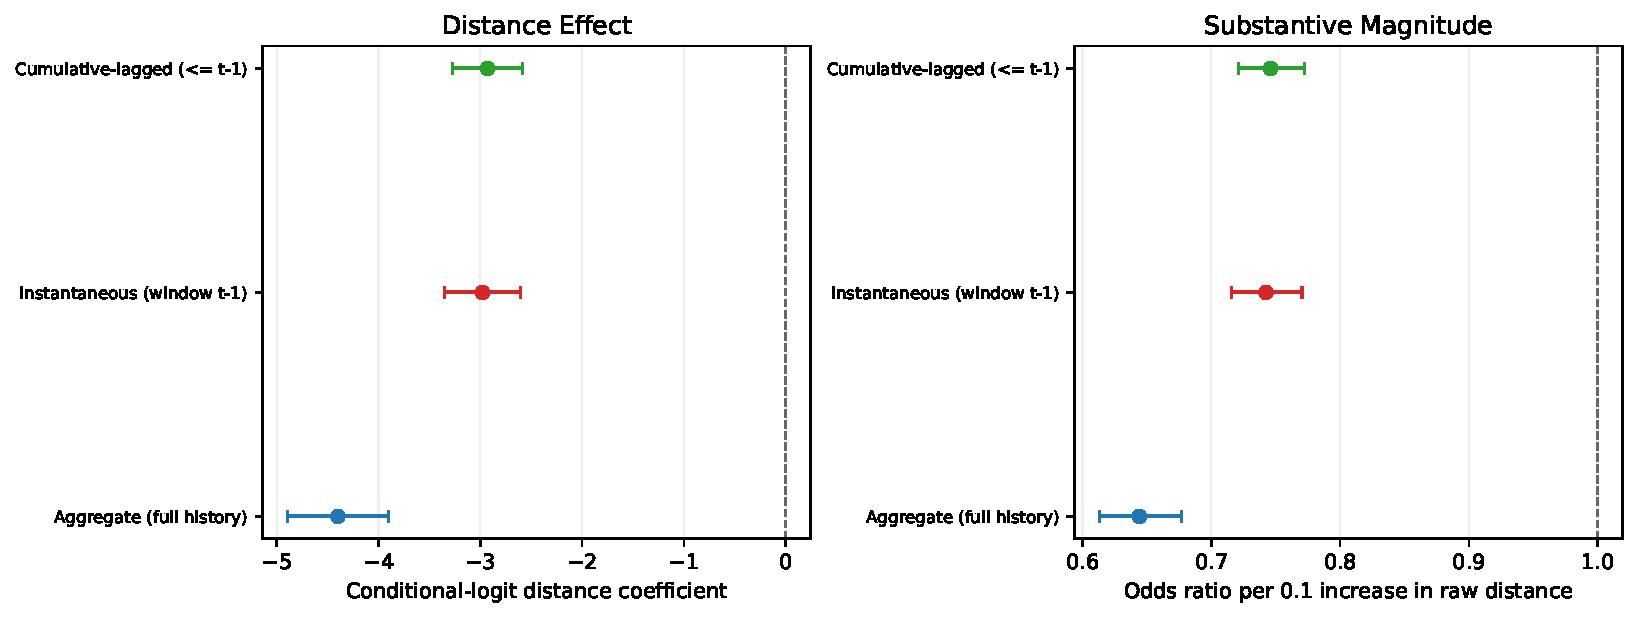
\includegraphics[width=\textwidth]{./figures/figS07_hazard_space_sensitivity.pdf}
\caption{\textbf{Local specialization persists across three temporal versions of the map.} Points are odds ratios for a $0.1$ increase in distance from the earlier portfolio. Bars are model-based 95\% intervals. The maps use the full archive, the previous five-meeting window, or all earlier records. Each model compares concerns available to the same actor at the same time and adjusts for prior popularity.}
 \label{fig:hazard-space-sensitivity}
\end{figure*}

One check changes the definition of the shift rather than the map. An actor can cross the RPA threshold because a concern becomes less common system-wide even when its own paper count does not rise. We therefore require that the actor filed no paper on the concern in the earlier window and at least one in the next. In the corresponding actor-period conditional model, moving $0.1$ farther gives an odds ratio of $0.874$ ($[0.834,0.916]$), close to the primary direction. \path{scripts/compare_major_results_category_treatments.py} reproduces the check.

Because each actor's submission history contributes to the proximities used to compute its distances, the locality test could contain a self-contribution. We therefore rebuild each actor's cumulative map without that actor while holding the prospective outcome panel fixed. We also divide each paper equally among its sponsors, in addition to dividing it among its categories. Both checks preserve the negative distance association. The prospective local result therefore does not depend on an actor contributing to its own map or on full co-sponsor credit. \path{scripts/hazard_circularity_checks.py} reproduces both analyses.

Although no edge is computed from text, the recovered geometry could still track the wording of the official labels. We compare the proximity matrix with TF-IDF cosine similarity over the same 45 labels, using word (1--2 gram, English stop words removed) and character (3--5 gram, word-boundary) analyzers. A Mantel permutation with $10{,}000$ joint row-and-column shuffles preserves dependence among the 990 pairwise entries. Lexical similarity is positively but weakly associated with proximity, explaining $0.9\%$ of its variance for word $n$-grams ($r=0.094$, Spearman $\rho=0.066$, $p=0.008$) and $1.5\%$ for character $n$-grams ($r=0.122$, $\rho=0.157$, $p=0.002$). This test does not remove concepts already built into the taxonomy; it shows only that literal label overlap explains little of the recovered co-specialization. \path{scripts/semantic_baseline.py} reproduces the numbers and pair table.

\begin{figure}
 \centering
 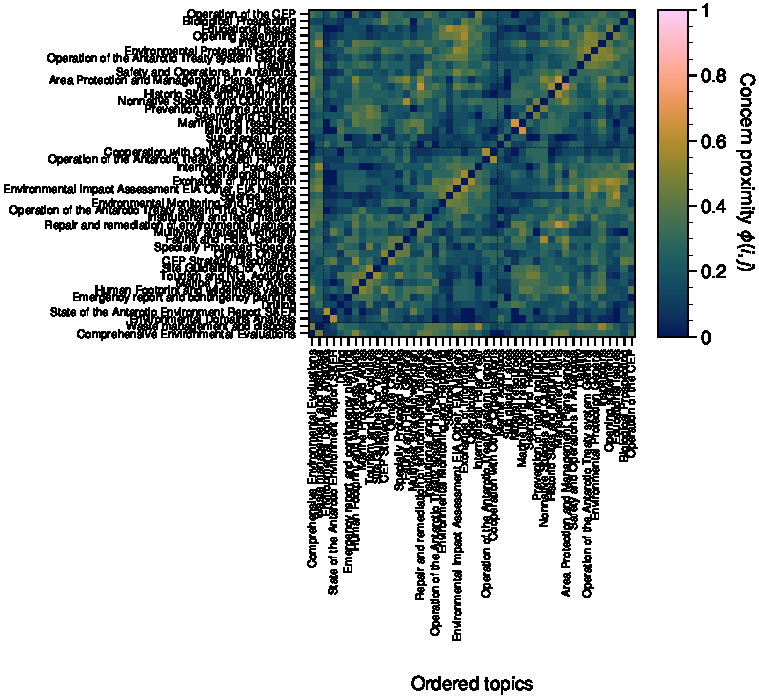
\includegraphics[width=0.45\textwidth]{./figures/figS09_concern_proximity_heatmap.pdf}
\caption{\textbf{Concern proximity is widespread but uneven.} Darker cells mark pairs more often held together in actors' specialized portfolios. Equation \cref{eq:proximity} defines the symmetric proximity measure.}
 \label{fig:heatmap_concerns}
\end{figure}

\subsection{A multiscale community reading}\label{sec:cpm-reading}
We use the Constant Potts Model (CPM) to summarize locally dense parts of the weighted concern network \cite{Traag2019}. CPM receives proximity $\phi$ directly as edge strength; it does not receive $1-\phi$ as a distance. At resolution $\gamma$, placing two concerns in the same community is favoured when their proximity exceeds $\gamma$ and penalized when it falls below $\gamma$. Sweeping $\gamma$ therefore reveals progressively finer readings rather than estimating one intrinsically correct number of communities.

The four-community reading at $\gamma=0.211$ contains groups of 30, 7, 5, and 3 concerns. The seven-community reading at $\gamma=0.273$ contains groups of 16, 13, 6, 4, 2, 2, and 2. The finer reading is mostly nested within the coarser one: 43 of 45 concerns fall within a single coarse parent, giving fine-to-coarse purity of $0.956$ (adjusted Rand index $0.478$; normalized mutual information $0.707$). The exceptions are Cooperation with Other Organisations and ATS reports, which form one fine pair across two coarse regions, and Marine Acoustics and Sub-glacial Lakes, which form another. \Cref{fig:cpm-partition-comparison} places both partitions on identical coordinates. \path{fig_cpm_partition_comparison.py} reproduces the comparison.

\begin{figure*}[!htbp]
 \centering
 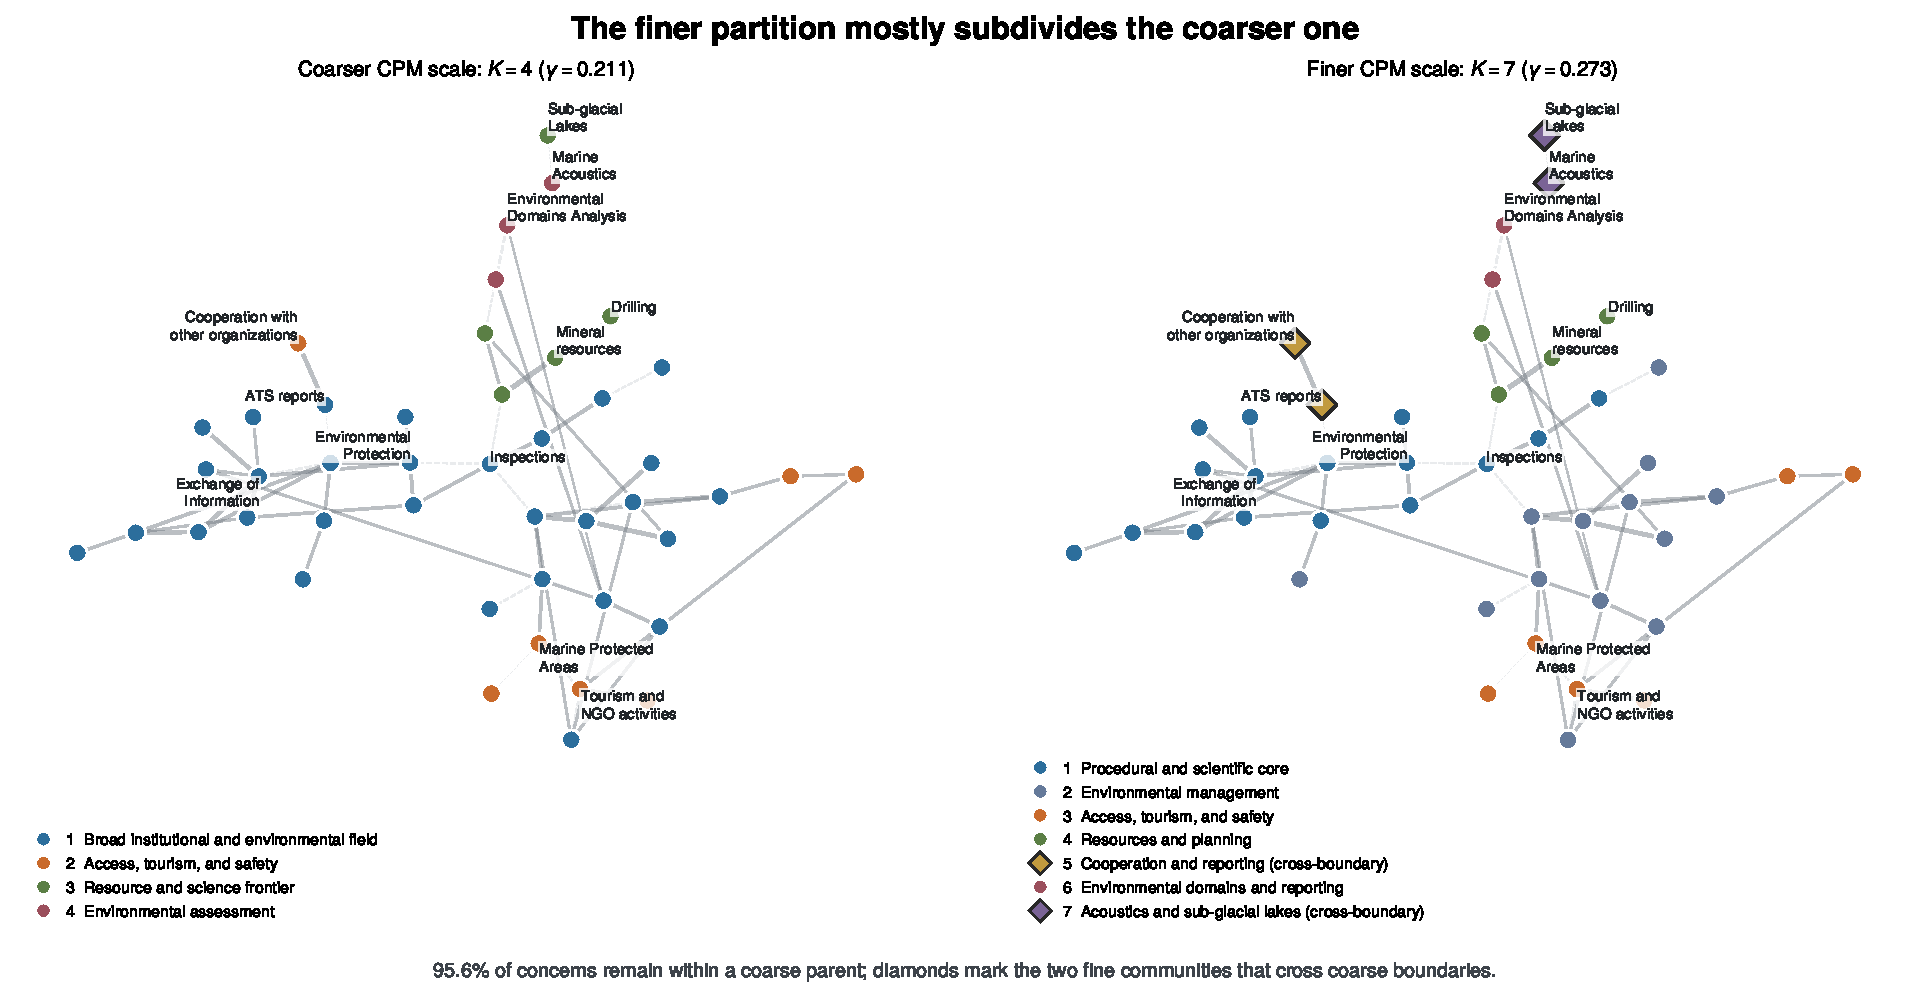
\includegraphics[width=\textwidth]{./figures/figS09a_cpm_partition_comparison.pdf}
 \caption{\textbf{Seven CPM regions mostly subdivide the four-region structure.} Both panels use the same nodes, edges, and coordinates. Related colours identify inherited coarse regions. Diamonds mark the two fine pairs that cross a coarse boundary. In total, $95.6\%$ of concerns remain within their fine region's majority coarse parent. Neither partition is uniquely identified.}
 \label{fig:cpm-partition-comparison}
\end{figure*}

To assess uncertainty, we resample submitting actors 300 times. Within every sample, we recompute RPA, rebuild the full proximity matrix, and refit CPM at $\gamma=0.273$. Pairwise co-assignment avoids matching arbitrary community numbers across bootstrap samples. The diagonal of \cref{fig:cpm-uncertainty} shows how often concerns from the same displayed region remain together; off-diagonal cells show merging across displayed regions. The pattern is dominated by internal subdivision rather than wholesale merging. The 16-concern procedural and scientific region has mean within-region co-assignment of $0.67$ but typically splits into three pieces. The 13-concern environmental-management region is less stable, with mean co-assignment of $0.41$. The small Cooperation--Reports and Environmental Domains--SAER pairs remain together in $79\%$ and $66\%$ of samples, while Marine Acoustics and Sub-glacial Lakes remain together in $40\%$. Because the probability that an entire region remains intact decreases mechanically with its size, we use pairwise co-assignment as the primary comparison. \path{scripts/analyze_cpm_partition_uncertainty.py} reproduces the bootstrap.

\begin{figure*}[!htbp]
 \centering
 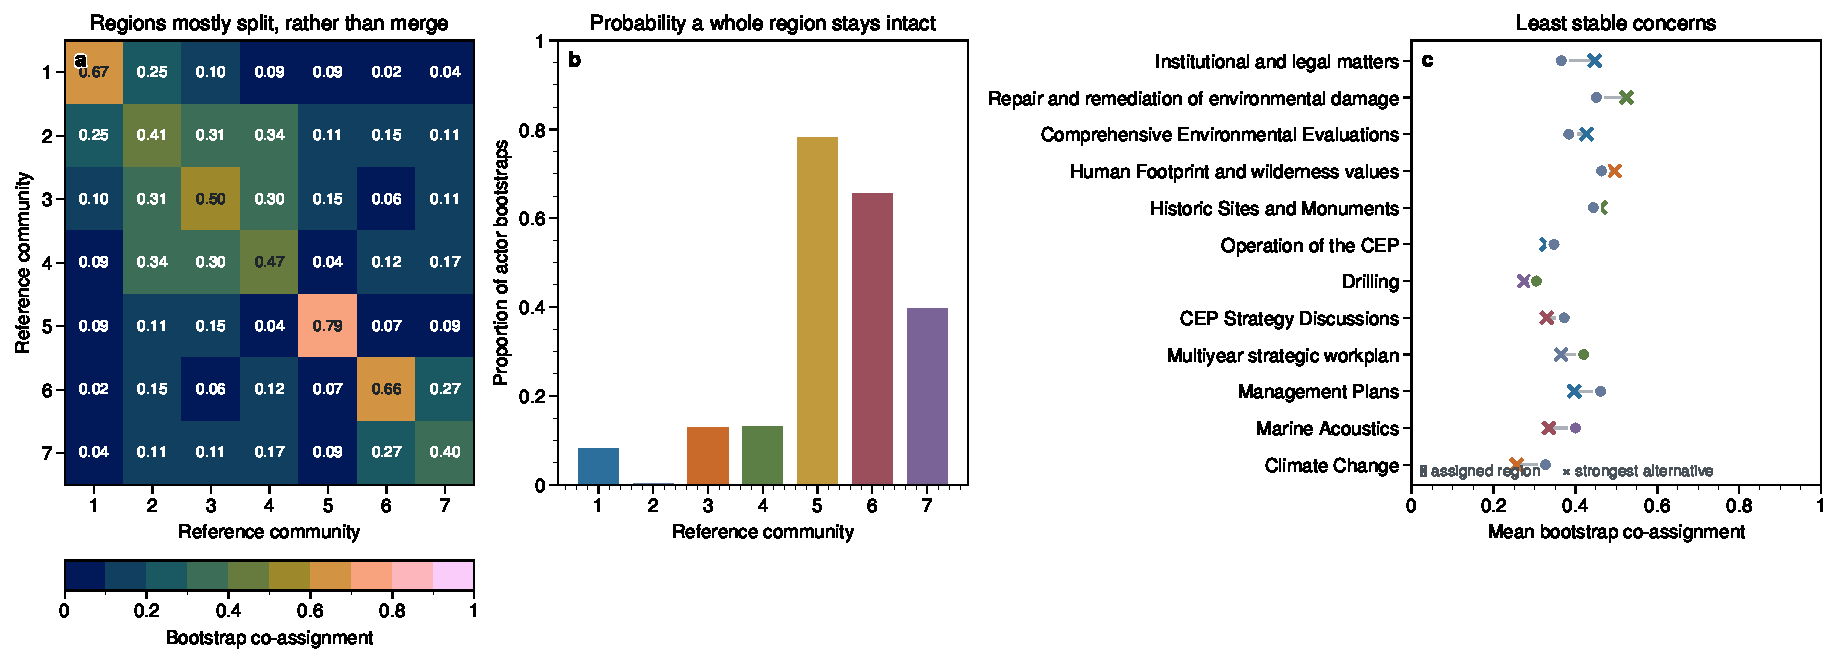
\includegraphics[width=\textwidth]{./figures/figS09b_cpm_k7_uncertainty.pdf}
 \caption{\textbf{Bootstrap variation divides broad regions more often than it merges them.} (a) Mean pairwise co-assignment across 300 actor bootstraps. Diagonal cells show persistence within displayed regions. Off-diagonal cells show merging between them. (b) Probability that an entire displayed region remains intact, a stricter measure that falls with region size. (c) The twelve concerns with the smallest margin between co-assignment with their displayed region (circle) and strongest alternative (cross).}
 \label{fig:cpm-uncertainty}
\end{figure*}

\subsection{Does any one actor determine the map?}\label{sec:space-robustness}
The space of concerns itself can be stress-tested by removing actors prior to construction and asking how much the resulting topic-topic proximity matrix changes. We proceed greedily by removing, at each step, the actor whose exclusion produces the largest root mean squared difference from the current full-space proximity matrix, then repeating the procedure. This does not test a substantive behavioral claim directly; it asks whether the shared topology of concerns is jointly produced or dominated by a small number of actors.

In \cref{fig:sensitivity-analysis}, the space changes gradually as actors are removed, indicating that the topology is not driven by one submitter. The comparison becomes less informative near the end of the sequence, when too few actors remain to estimate the original links. This test shows that the pooled map draws on many submitters; it does not establish that individual edge ranks or the map remain fixed over time.

\begin{figure}
 \centering
 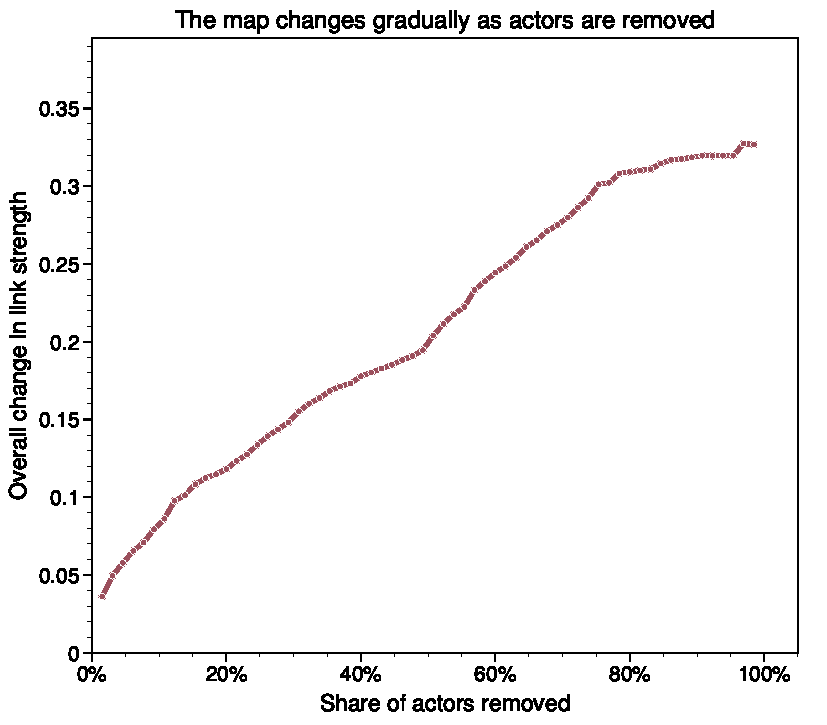
\includegraphics[width=0.45\textwidth]{./figures/figS10_space_member_removal.pdf}
 \caption{\textbf{No single actor determines the concern map.} At each step, the actor whose removal changes the map most is excluded and the map is rebuilt. The vertical axis is the root mean squared change across all links. Change accumulates gradually rather than appearing after one removal. The undefined comparison after the final actor is omitted is not shown.}
 \label{fig:sensitivity-analysis}
\end{figure}

\subsection{Placing formal outcomes in the concern space}\label{sec:outcome-positioning}
The output inventory contains all 584 records with titles from regular ATCMs 19--47 (1995--2025): 277 Measures, 135 Decisions, and 172 Resolutions. We begin in 1995 because Decision 1 (1995) established these output types and the official register is complete for the period. Measures become legally binding after the required approvals. Decisions address internal organizational matters and are operative on adoption or another stated date. Resolutions are hortatory and not legally binding. We therefore pool them only as \emph{adopted ATCM outputs}; the count does not imply equal legal effect. Instruments adopted at Special ATCMs, including the 1991 Madrid Protocol, are outside this inventory. Each record retains instrument type, number, year, and meeting because numbers repeat across years. The analysis reads these records directly from the archived 9 February 2026 official export and verifies its SHA-256 checksum, total counts, type counts, and counts by meeting.

The official instrument register supplies a Category field for every retained output. Its 15 broad categories do not correspond one-to-one with the 45 finer paper concerns. We therefore place every paper concern within one broad output family and rebuild the paper map at that common resolution. For a paper returned under several fine concerns, its fractional weights are summed within families and still total one. Sixty outputs have more than one official category, giving 646 output--category relations; an output with $k$ categories contributes $1/k$ to each. The resulting weights also total one for every output.

This 45-to-15 hierarchy is an author-coded analytic device, not a Secretariat crosswalk. It groups concerns by the scope of the official output categories. For example, Management Plans, Environmental Domains Analysis, Marine Protected Areas, and the general area-protection concern all enter ``Area protection and management''. The complete hierarchy is shown in \cref{tab:output-category-crosswalk}. \path{scripts/official_regular_atcm_outputs.py} freezes the mapping, and \path{scripts/analyze_output_category_families.py} rebuilds the broad paper map and output analysis.

\begin{table*}[!htbp]
\centering
\scriptsize
\caption{\textbf{Paper concerns are grouped into the 15 official output categories.} The left column lists categories from the ATS instrument register. The right column lists the paper concerns assigned to each for analysis. This author-coded hierarchy is not an official Secretariat crosswalk.}
\label{tab:output-category-crosswalk}
\begin{tabular}{@{}p{0.39\textwidth}p{0.53\textwidth}@{}}
\toprule
Official instrument category & Included paper concerns \\
\midrule
Area protection and management & Area Protection and Management Plans General; Management Plans; Environmental Domains Analysis; Marine Protected Areas \\
Institutional \& legal matters & Operation of the ATS: General, Reports, and Secretariat; Cooperation with Other Organisations; Liability; Institutional and legal matters; Multiyear strategic workplan \\
Tourism and Non-Governmental Activities & Tourism and NG Activities; Site Guidelines for Visitors \\
Operational matters & Inspections; Search and Rescue; Operational issues; Safety and Operations in Antarctica; Emergency report and contingency planning \\
Environmental protection & Climate Change; Environmental Protection General; Environmental Monitoring and Reporting; CEP Strategy Discussions; Human Footprint and wilderness values; Operation of the CEP; State of the Antarctic Environment Report; Repair and remediation of environmental damage \\
Historic Sites and Monuments & Historic Sites and Monuments \\
Information exchange & Exchange of Information \\
Scientific cooperation & Science issues; Marine Acoustics; International Polar Year; Sub-glacial Lakes; Drilling; Biological Prospecting \\
Fauna and flora & Fauna and Flora General; Specially Protected Species; Nonnative Species and Quarantine \\
Marine pollution & Prevention of marine pollution \\
Environmental impact assessment & Environmental Impact Assessment: Other EIA Matters; Comprehensive Environmental Evaluations \\
General matters & Educational issues; Opening statements \\
Marine living resources & Marine living resources \\
Waste disposal and management & Waste management and disposal \\
Mineral resources & Mineral resources \\
\bottomrule
\end{tabular}
\end{table*}

\subsection{Prospective forecasts of formal output}\label{sec:prospective-output-forecast}
We test whether papers help locate formal output before it is adopted. The target is not the total number of instruments. For each output type and rolling-origin test meeting, it is the distribution of that meeting's output weight across the 15 official categories. If output $r$ at meeting $t$ assigns observed share $q_{irt}$ to category $i$, and a model assigns predicted share $\widehat{p}_{irt}$, we score the forecast as
\begin{equation}
 \mathcal{L}_{rt}=-\sum_i q_{irt}\log \widehat{p}_{irt}.
\end{equation}
Lower values mean that the model placed more probability on the categories where output was adopted.

For the redesigned specification, we use pooled Measures, Decisions, and Resolutions from ATCMs 25--28 to select among output-history windows of 3, 5, 8, or 10 meetings, direct-attention windows of 1, 2, 3, or 5 meetings, and regularization values of $0.1$, $0.2$, $0.5$, or $1.0$. This selects five meetings of output history, one meeting of earlier direct attention, and regularization $0.1$. We freeze those settings and run a rolling-origin evaluation on ATCMs 29--47, giving 19 test meetings for each output type. At each test meeting, the model is fitted on ATCM 20 through the meeting immediately before it. A regularized Poisson model includes category indicators and standardized numerical features; predictions are normalized across categories before scoring. Earlier exploratory versions of the analysis had already examined ATCMs 29--47, so this period is a prospective test within each meeting but not an untouched external validation.

The benchmark contains the preceding five meetings of the same output type in the category. The direct-attention model adds fractionally counted papers and the number of distinct submitting actors in the category during the immediately preceding meeting, plus the same two quantities for the focal meeting. Papers submitted for the focal ATCM are inputs to that meeting and are observable before its outputs are adopted. The exercise is therefore a pre-adoption nowcast, not a forecast made years in advance. The full model adds current paper attention in every positively connected non-focal broad category, up to 14. For each target category, the pre-meeting proximities are normalized to one and applied to focal-meeting paper counts. This network extension introduces no chosen neighbourhood size. The broad map is rebuilt from papers submitted before the focal meeting.

We compare models within each test meeting and resample the 19 paired score differences 20,000 times to form 95\% intervals. Output-type contrasts resample the paired difference between Resolution gains and the corresponding Measure or Decision gains. Robustness checks vary the output-history window, direct-attention window, regularization, and number of neighbours; omit each target category from scoring in turn; replace network attention with all other papers; project current papers through the original 45-concern map; split the test period; and use moving-block meeting bootstraps. A nested rolling-origin check reselects every setting using only meetings before each test meeting.

As a post hoc concentration check, we calculate the Shannon entropy of the adopted Resolution distribution within each test meeting and split the 19 meetings at the median. We report the mean score change in each half, their difference, and the correlation between score change and entropy. Intervals resample meetings within each half. This check asks whether the gain is confined to meetings with unusually broad Resolution output; it does not make Measures, Decisions, and Resolutions compositionally equivalent. \path{scripts/analyze_resolution_concentration_sensitivity.py} reproduces the calculation.

The geometry null uses 200 label permutations. At each meeting, it applies the same permutation to the rows and columns of the pre-meeting proximity matrix, recomputes the network-weighted paper counts, and refits every forecast. The test therefore breaks which categories occupy neighbouring positions while preserving a coherent symmetric map. Because lower score changes are better, its lower-tail probability is $(1+b)/(1+200)$, where $b$ counts shuffled changes less than or equal to the observed change. The Area protection and management check omits that target row from scoring but leaves its papers available as network attention for other categories. \path{scripts/analyze_resolution_attention_forecast.py} reproduces the primary forecasts and checks; \path{scripts/evaluate_nested_attention_forecast.py} reproduces the within-fold selection sensitivity.

\subsection{Auditing formal inheritance among Measures}\label{sec:formal-inheritance-audit}
The forecast asks whether attention helps locate adopted output. A separate audit asks what formal record later Measures cite. We froze the adopted body text from the official detail page of every one of the 277 Measures on 16 August 2026. The pinned JSONL corpus records each official URL, retrieval date, extraction status, and body hash; an adjacent manifest records the corpus SHA-256 and verifies the source inventory and all 277 records. The audit consumes this corpus without live requests. We extract exact references of the form \emph{Measure}, \emph{Decision}, or \emph{Resolution} followed by a number and year. Instrument numbers restart each year, so type, number, and year jointly identify every source. A reference counts only when it resolves to an earlier entry in the pinned official inventory. Repeated mentions of the same source within one Measure count as one link.

The audit reports the number of later Measures citing each source type, the number of distinct earlier instruments cited, and the number of source--Measure links. A later Measure can cite several source types, so the percentages in \cref{fig:selective-translation}b overlap. These exact references are a conservative trace of formal inheritance. They do not establish that the earlier instrument caused the later one, and a policy sequence can omit an intermediate source from its final adopted body text. We also screen Measure titles for ``management plan'' and ``revised management plan'' to describe the recurring content of the Measure record.

To examine whether heavily discussed Resolutions are the ones that later enter a Measure, we retain Resolutions with ten subsequent regular meetings in the archive. A Resolution enters the linked set only when a Measure adopted within those ten meetings contains an exact year-qualified citation to it. For each linked Resolution, we compare same-category paper attention with uncited Resolutions sharing at least one official category and report its percentile within that set. Time is counted in meetings rather than calendar years. The linked sample is small, so this is a descriptive boundary test rather than a fitted transition model. \path{scripts/audit_resolution_measure_ladders.py} and \path{scripts/analyze_resolution_hardening_attention.py} reproduce the audit.

\subsection{Pooled paper--output associations as a boundary test}\label{sec:attention-output-models}
The category--meeting analysis orders the record by ATCM number, so one step is the immediately preceding meeting even when more than one calendar year elapsed. For broad category $i$ at ATCM $t$, we measure three earlier histories: fractionally counted papers in $i$; papers in its five nearest broad categories, weighted using the map available before each source meeting; and adopted outputs in $i$. For the primary one-meeting analysis, each history comes from ATCM $t-1$, and its nearby-paper weights use the map built through $t-2$. We add one and take the logarithm.

A Poisson pseudo-maximum-likelihood model uses category and meeting fixed effects. The reported rate ratios give the change associated with doubling one plus an earlier count. Covariance is clustered by category and meeting. Because there are only 15 category clusters, the intervals should be read cautiously. They also condition on the author-coded hierarchy and estimated map; uncertainty in those objects is not propagated.

We repeat the analysis after combining the preceding one, two, three, five, eight, or ten meetings. The available meeting set therefore shrinks as the window grows. To separate window length from sample period, we repeat every horizon on the 19 meetings shared by the ten-meeting model (ATCMs 29--47). Composition checks exclude General matters, Area protection and management, or both. The latter matters because recurring area and management-plan work makes up almost half of the adopted-output category weight. All comparisons describe temporal association between documentary streams and adopted outputs, not a causal effect of papers on output. \path{scripts/analyze_output_category_families.py} reproduces the models.

\section{Supplementary Results}
\subsection{Forecast performance differs by output type}\label{sec:forecast-results}
The rolling-origin comparison separates the direct and network components of the attention model (\cref{tab:output-forecast-scores}). Their combined change improves the Resolution forecast relative to output history. The intervals for the two components considered separately cross zero. Neither the combined model nor its direct component improves the Measure or Decision forecast. The complete Resolution gain is larger than the Measure gain by $0.063$ ($[-0.112,-0.012]$) and larger than the Decision gain by $0.092$ ($[-0.159,-0.022]$).

\begin{table*}[!htbp]
\centering
\scriptsize
\caption{\textbf{Attention improves Resolution forecasts but not Measure or Decision forecasts.} Entries are mean changes in allocation log score with meeting-bootstrap 95\% intervals. Negative values improve prediction. The first two columns compare attention models with output history. The final column adds network-weighted attention to direct attention.}
\label{tab:output-forecast-scores}
\begin{tabular}{@{}lccc@{}}
\toprule
Output type & Direct vs history & Direct + network vs history & Network vs direct \\
\midrule
Measure & $0.007$ $[-0.012,0.025]$ & $-0.001$ $[-0.023,0.020]$ & $-0.008$ $[-0.015,-0.001]$ \\
Decision & $0.024$ $[-0.023,0.069]$ & $0.028$ $[-0.022,0.075]$ & $0.003$ $[-0.002,0.009]$ \\
Resolution & $-0.041$ $[-0.082,0.001]$ & $-0.065$ $[-0.114,-0.014]$ & $-0.023$ $[-0.050,0.002]$ \\
\bottomrule
\end{tabular}
\end{table*}

The output types pose different prediction problems. The effective number of occupied categories, calculated as the exponential of Shannon entropy, is 10.55 for Resolutions, 3.14 for Decisions, and 1.38 for Measures. Area protection and management accounts for $93.1\%$ of fractional Measure weight, while Institutional and legal matters accounts for $73.0\%$ of Decision weight. The largest Resolution category, Tourism and Non-Governmental Activities, accounts for only $22.1\%$. Earlier output is therefore already a strong guide to the narrow Measure and Decision distributions.

Within the 19 Resolution test meetings, the combined score change is $-0.073$ in the ten meetings at or below median category entropy ($[-0.141,-0.006]$) and $-0.055$ in the nine meetings above it ($[-0.125,0.021]$). Their difference is $0.018$ ($[-0.080,0.119]$). The correlation between score change and entropy is $-0.043$ ($[-0.417,0.318]$). The point estimates do not suggest that the Resolution gain is created by the broadest meetings, but the intervals remain wide.

For Measures, using prior Measures alone gives a mean rolling-origin score of $0.388$. Prior Decisions and Resolutions alone score $1.134$, all earlier output scores $0.486$, and direct plus network attention without Measure history scores $0.759$. Adding Decisions and Resolutions to prior Measures worsens the score by $0.011$ ($[0.000,0.023]$). Adding attention to prior Measures changes it by $-0.001$ ($[-0.023,0.020]$). The recurrence is consistent with the content of the record: 266 of 277 Measures carry the Area protection and management category, 230 titles concern a management plan, and 211 concern a revised management plan.

The Resolution result is not reproduced by generic activity outside the focal category. Adding all other papers to the direct-attention model changes the score by $0.001$ ($[-0.001,0.003]$), compared with $-0.023$ for network-weighted papers. Omitting each broad category from the score leaves the mean network gain negative in all 15 cases, ranging from $-0.033$ to $-0.016$. Every one of the 16 combinations of output-history and attention windows gives a negative mean gain, as do all five tested neighbour counts and all four regularization values. All six projections through the original 45-concern map improve the mean score. Moving-block bootstraps of one to four meetings preserve the negative mean, although their intervals cross zero. The gain is $-0.008$ in ATCMs 29--38 ($[-0.038,0.025]$) and $-0.040$ in ATCMs 39--47 ($[-0.083,-0.005]$). When every setting is instead reselected within each rolling training period, the combined Resolution change remains similar at $-0.067$, but its interval crosses zero ($[-0.131,0.004]$). We use the fixed early-period specification as the primary summary because its settings are transparent and shared across output types; the nested result shows that model selection adds uncertainty without reversing the mean pattern.

\subsection{Measures inherit a narrow formal record}\label{sec:formal-inheritance-results}
The adopted body text of 245 of 277 Measures cites at least one earlier Measure, Decision, or Resolution (\cref{tab:measure-formal-inheritance}). Prior Measures provide the broadest source set: 173 distinct earlier Measures appear in 474 links to 231 later Measures. The 261 Decision links come from only eight distinct Decisions, showing repeated use of a small administrative foundation. Nine distinct Resolutions appear in 81 links to 73 Measures.

\begin{table*}[!htbp]
\centering
\scriptsize
\caption{\textbf{Measures cite earlier Measures more widely than Decisions or Resolutions.} Links require an exact, year-qualified reference in a later Measure's adopted body text and a match to the official inventory. Rows overlap because a Measure can cite several source types. Lag is measured in calendar years.}
\label{tab:measure-formal-inheritance}
\begin{tabular}{@{}lrrrr@{}}
\toprule
Earlier output type & Later Measures citing type & Distinct earlier outputs & Citation links & Median lag \\
\midrule
Measure & 231 & 173 & 474 & 8 \\
Decision & 171 & 8 & 261 & 11 \\
Resolution & 73 & 9 & 81 & 18 \\
\bottomrule
\end{tabular}
\end{table*}

The Resolution links are concentrated in established administrative sequences. Eighty of 81 concern protected-area or heritage work. Repeated Measures cite Resolutions that set expiry rules, management-plan formats, revision responsibilities, or heritage-assessment procedures. Resolution 4 (2007) on ship-based tourism and Measure 15 (2009) on passenger-vessel landings form the only cited pair outside those domains.

Exact citations miss intermediate steps that the final Measure does not repeat. Decision 3 (1998) moved further negotiation of a liability annex to ATCM Working Group I, Resolution 5 (1999) requested practical and scientific input, Decision 3 (2001) advanced a draft, Measure 1 (2005) adopted Annex VI, and Decision 1 (2005) established annual review of progress towards its becoming effective. The 2005 Measure does not cite the 1999 Resolution. For this reason, \cref{tab:measure-formal-inheritance} is a lower bound on documented continuity and not a complete lineage reconstruction.

Only six of the 115 Resolutions with ten subsequent meetings available are cited by a Measure within that period. Their same-category paper attention is not unusually high relative to uncited Resolutions sharing an official category. The linked Resolutions average the 24th percentile for the current and two preceding meetings, then the 33rd, 36th, 39th, 42nd, and 43rd percentiles after one, three, five, eight, and ten meetings. The sample is too small for a general transition model, but it does not support a simple rule in which the most heavily discussed Resolutions enter the Measure track. Entry into that track also does not establish that the later Measure entered into force.

\subsection{The paper--output association changes with sample period}\label{sec:attention-accumulation-results}
At the immediately preceding ATCM, doubling one plus papers in the same broad category is associated with an output-rate ratio of $1.189$ ($[1.036,1.364]$). The corresponding estimate for papers in the five nearest categories is $0.989$ ($[0.926,1.055]$), and that for earlier output in the same category is $1.396$ ($[1.162,1.677]$). The ratio between the same-category and nearby-paper rate ratios is $1.202$ ($[1.023,1.413]$, $p=0.025$). The nearby estimate is conditional on same-category papers and should not be read as evidence that neighbouring attention suppresses output.

Changing the window also changes which meetings can enter the model. With every eligible meeting included, the same-category versus nearby contrast is clear at one meeting ($1.202$, $[1.023,1.413]$) and three meetings ($1.304$, $[1.032,1.648]$), but not at five meetings ($1.391$, $[0.936,2.067]$). Over the same 19 later meetings, the corresponding contrasts are $0.922$ ($[0.699,1.216]$), $0.961$ ($[0.671,1.375]$), and $0.979$ ($[0.577,1.662]$). None of the common-support estimates from one to ten meetings is clear. The full-record result therefore varies with sample period rather than identifying a fixed lag or cumulative conversion law.

Composition changes the precision of the result. After removing Area protection and management from the paper histories, broad map, and output panel, the one-meeting contrast is $1.309$ ($[0.997,1.719]$); after also removing General matters, it is $1.230$ ($[0.853,1.774]$). The point estimates do not shrink, so these checks do not show that area management creates the association. They do show that the full-record contrast is no longer clear once the dominant family is removed. Almost half of output category weight belongs to area protection and management, much of it recurring site and management-plan work.

\begin{figure*}[!htbp]
\centering
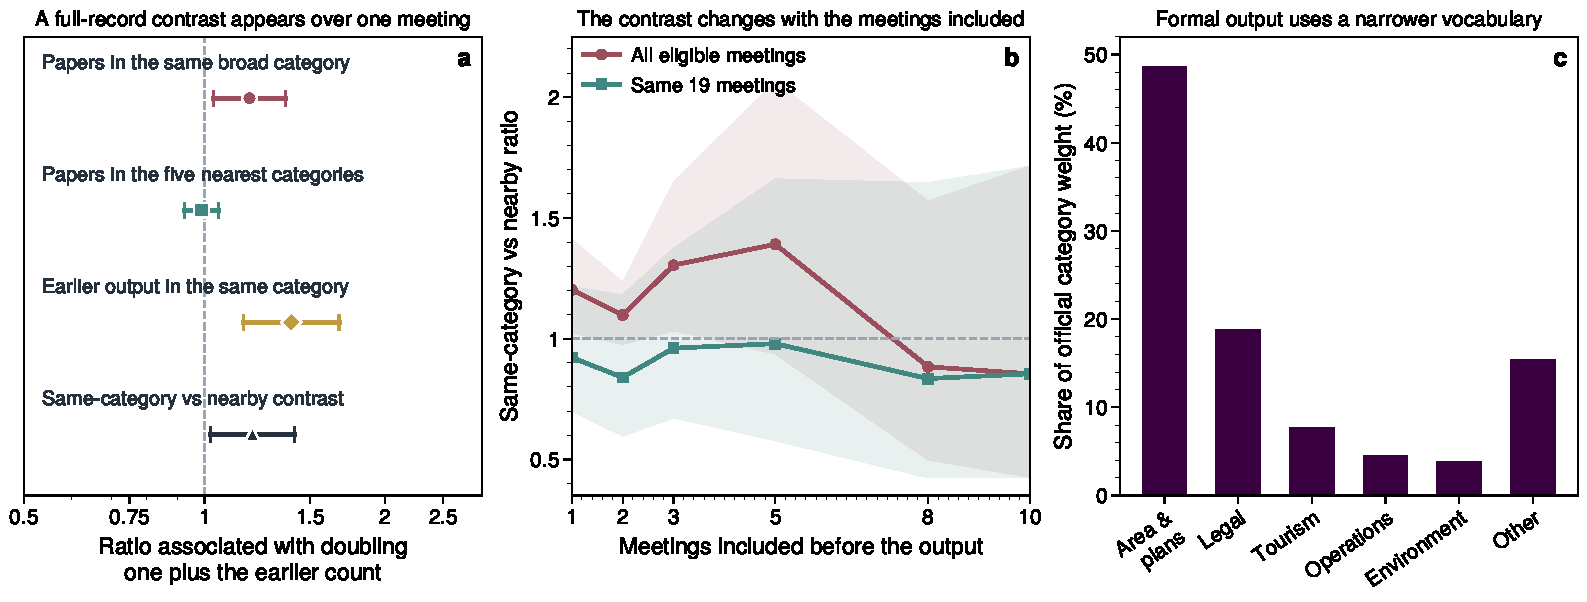
\includegraphics[width=\textwidth]{figures/fig03_selective_translation.pdf}
\caption{\textbf{The pooled association between papers and outputs changes with sample period.} (a) Output-rate ratios for the immediately preceding ATCM. The fourth estimate compares the same-category and nearby-paper rate ratios. Bars are two-way-clustered 95\% intervals. (b) That contrast across one to ten preceding meetings, using either every eligible meeting or the same 19 later meetings. (c) Composition of the pooled output record. Because this boundary test combines Measures, Decisions, and Resolutions, it does not estimate the type-specific forecast result in \cref{fig:selective-translation}.}
\label{fig:pooled-output-boundary}
\end{figure*}

\subsection{Where later entrants begin}\label{sec:secondary-structure-results}

In a retrospective pooled-map comparison, actors joining in 1991--2010 ($n=17$) built opening portfolios around concerns whose full-record holders covered fewer concerns than expected ($0.929\times$ the career-stage benchmark; 95\% actor-bootstrap interval $[0.889,0.966]$). Those concerns also have fewer pooled-map neighbours on average ($0.883\times$ the benchmark, $[0.798,0.974]$). Earlier cohorts sit near parity on both measures. The full estimates and construction are in \cref{sec:cohort-method,tab:cohort-ratios}. This selected comparison excludes post-2010 entrants by design, conditions eligibility on a 15-year record, and does not reconstruct the information set available at entry.

\subsection{Alternative matched comparisons}\label{sec:paired-null-robustness}
The paired test compares each realized specialization shift with a size-matched redraw from concerns the actor did not hold. We vary the pooled or cumulative-lagged map, uniform or popularity-weighted redraws, and whether candidates are drawn from all eventual labels, those observed by the current-window end, or those observed before the transition. Popularity weights equal the number of actors specialized in the concern in the previous window plus one. Each event uses 200 redraws.

Every construction places realized shifts nearer than its null more often than not. The primary prospective comparison uses the cumulative-lagged map, prior popularity, and only concerns already observed before the transition. It contains 968 actor-periods and gives $62.5\%$ nearer (95\% actor-bootstrap interval $[58.9,66.5]\%$). The observed median displacement is $0.576$, against a weighted-alternative median of $0.594$ ($p=1.3\times10^{-15}$ in the unclustered Wilcoxon comparison). \path{scripts/compare_major_results_category_treatments.py} reproduces the comparison and actor bootstrap.

\begin{table*}[!htbp]
\centering
\scriptsize
\caption{\textbf{Local specialization persists across alternative comparisons.} Each row changes the comparison, outcome, category treatment, or time window. OR is the change in crossing odds for a $0.1$ increase in distance from the earlier portfolio. The final row separately summarizes specialization duration.}
\label{tab:locality_estimands}
\begin{tabular}{@{}p{0.30\textwidth}p{0.22\textwidth}p{0.40\textwidth}@{}}
\hline
\textbf{Comparison} & \textbf{Result} & \textbf{Question answered} \\
\hline
Prospective popularity-weighted alternatives ($n=968$) & 62.5\% nearer, actor-bootstrap interval $[58.9,66.5]\%$ & Is the realized specialization shift nearer than alternatives weighted by their earlier popularity? \\
\hline
Prospective within-actor model (30,957 available concerns) & OR $0.817$ $[0.783,0.853]$ per $0.1$ farther & Among options open to the same actor at the same time, are nearby concerns more likely to cross the threshold? \\
\hline
First-paper outcome and one-category robustness & OR $0.874$ $[0.834,0.916]$ and $0.831$ $[0.794,0.870]$ & Does the direction remain after changing the outcome or forcing one inferred category per paper? \\
\hline
Disjoint five-meeting windows & OR $0.904$ $[0.855,0.957]$ & Does the adjacent-window result extend to non-overlapping blocks? \\
\hline
Years active after a concern first enters & 5--42\% remain after ten years and fewer than 20\% after twenty years, depending on whether a lapse of one to five years is allowed & How much does the length of apparent specialization depend on the rule for a temporary lapse? \\
\hline
\end{tabular}
\end{table*}

\FloatBarrier

\subsection{A boundary test: the 1991 Madrid Protocol}\label{sec:madrid-shock}

To ask whether pre-shock position also predicts responses outside routine portfolio evolution, we examine the reorientation surrounding the 1991 Madrid Protocol. The Convention on the Regulation of Antarctic Mineral Resource Activities (CRAMRA) was adopted in Wellington in 1988 and abandoned after Australia and France declined to sign it in 1989; the Protocol negotiations of 1989--91 replaced it \cite{Joyner1998}. The documentary record in 1986--90 therefore contains attention to the failed instrument as well as the concerns later reorganized by the Protocol.

Using pre-1991 inputs where possible, the design defines the boosted set as the eight concerns whose share of the archive grew most between 1986--90 and 1992--96. We restrict it to concerns with at least $1\%$ pre-presence so that categories created by the Protocol itself cannot enter. Adjacency is the maximum proximity between an actor's pre-1991 portfolio ($RPA \ge 1$) and the boosted set, estimated on 1961--90 documents only. The outcome is the share of an actor's papers in each 5-year window that falls in the boosted set, modeled with window dummies interacted with adjacency, actor and window fixed effects, window-by-portfolio-size controls, and actor-clustered standard errors (30 actors, 263 actor-window observations with at least three papers).

The pre-period coefficients do not reject parallel trends (joint $F(5,\cdot)=1.61$, $p=0.159$), although this low-powered diagnostic does not establish that the shock is exogenous. Every post-shock adjacency-by-window coefficient is negative and small relative to its uncertainty (range $-0.83$ to $-0.19$ percentage points). A second-pass model asks whether an actor's adjacency to the Protocol's compliance set predicts entry into that set; its coefficient is also negative and uncertain ($-3.02$, SE $3.12$, $p=0.334$). Adjacency is strongly correlated with pre-1991 portfolio size ($r=0.87$), which the window-by-portfolio-size controls absorb.

The null does not refute the routine predictive association, but it fails to extend that association to an unusually large institutional reorientation. Pre-shock position did not discriminate who responded, and the design cannot determine whether the collective response overrode a normally local process or arose through a different process altogether. We report this exploratory boundary test because its outcome limits the mechanism reading of the main text. \path{scripts/madrid_shock_exploration.py} reproduces the analysis.

\end{document}
